%%%%%%%%%%%%%%%%%%%%%%% file template.tex %%%%%%%%%%%%%%%%%%%%%%%%%
%
% This is a general template file for the LaTeX package SVJour3
% for Springer journals.          Springer Heidelberg 2006/03/15
%
% Copy it to a new file with a new name and use it as the basis
% for your article. Delete % signs as needed.
%
% This template includes a few options for different layouts and
% content for various journals. Please consult a previous issue of
% your journal as needed.
%
%%%%%%%%%%%%%%%%%%%%%%%%%%%%%%%%%%%%%%%%%%%%%%%%%%%%%%%%%%%%%%%%%%%
%
% First comes an example EPS file -- just ignore it and
% proceed on the \documentclass line
% your LaTeX will extract the file if required
%\begin{filecontents*}{example.eps}
%%%!PS-Adobe-3.0 EPSF-3.0
%%%BoundingBox: 19 19 221 221
%%%CreationDate: Mon Sep 29 1997
%%%Creator: programmed by hand (JK)
%%%EndComments
%gsave
%newpath
%  20 20 moveto
%  20 220 lineto
%  220 220 lineto
%  220 20 lineto
%closepath
%2 setlinewidth
%gsave
%  .4 setgray fill
%grestore
%stroke
%grestore
%\end{filecontents*}
%
%\documentclass{svjour3}                     % onecolumn (standard format)
%\documentclass[smallextended]{svjour3}     % onecolumn (second format)
%\documentclass{svjour3}        % twocolumn
\documentclass[smallcondensed]{svjour3} %requested in Journal 
\smartqed  % flush right qed marks, e.g. at end of proof
%


\usepackage{graphicx}
\usepackage{palatino,epsfig,latexsym}
\usepackage{amsmath,amsfonts,amssymb,color}
\usepackage{graphicx}
\usepackage{algorithm}
\usepackage{algorithmic}
\usepackage{subfigure}
\usepackage{multirow}
\usepackage{bbm}
\usepackage{url}
\usepackage{float}
\renewcommand{\textfraction}{.01}
\renewcommand{\bottomfraction}{.99}
\renewcommand{\topfraction}{.99}
%\setcitestyle{square}
\sloppy
%
\begin{document}

\title{EvoSpace: A framework for Pool-Based Evolutionary Algorithms}
% a framework that does what? That is the best for what? Is this a
% publicity paper or something more? What are you going to say about
% this framework? Introducing? Assessing? - JJ


%\titlerunning{Short form of title}        % if too long for running head

\author{Mario Garc\'ia-Valdez         \and
        Leonardo Trujillo \and
		Juan-J Merelo\and
		Francisco Fern\'andez-de-Vega\and
		Gustavo Olague
		}

%\authorrunning{Short form of author list} % if too long for running head

\institute{Mario Garc\'ia-Valdez \at
           Instituto Tecnol\'ogico de Tijuana, Calzada Tecnol\'ogico S/N, Tijuana, BC, 22414  \\	
              \email{mario@tectijuana.edu.mx}           %  \\
%             \emph{Present address:} of F. Author  %  if needed
           \and
           Leonardo Trujillo \at
           \email{leonardo@tectijuana.edu.mx}  
			\and
			Juan-J Merelo
	         \at
	        Departamento de Arquitectura y Tecnolog\'ia de Computadores University of Granada, Spain\\
	\email{jmerelo@geneura.ugr.es}
			\and
			Francisco Fern\'andez-de-Vega
			\at
			Grupo de Evoluci\'on Artificial, Universidad de Extremadura, Spain\\
	\email{fcofdez@unex.es}	
		\and
		Gustavo Olague
		\at
		Centro de Investigaci\'on Cient\'ifica y de Educaci\'on Superior de Ensenada\\
\email{olague@cicese.mx}		
}

%\date{Received: date / Accepted: date}
% The correct dates will be entered by the editor


\maketitle

\begin{abstract}


\keywords{Pool-based Evolutionary Algorithms \and Distributed Evolutionary Algorithms\and Heterogeneous Computing Platforms for Bioinspired Algorithms  \and Parameter Setting}

\end{abstract}

\section{Introduction}
\label{sec:intro}
%Over the last decade,  %I'd change that to concrete dates. Nobody
                       %knows $n$ years from now which decade was that
                       %- JJ
%the landscape in computing technology has undergone a noticeable shift, moving away from isolated,
%serial, single-tenant and synchronous systems, towards distributed,
%ubiquitous, multi-tenant and shared computing resources,
%exploiting network infrastructure and what is known as the Cloud Computing model\cite{cloud, varia2008cloud}.
%This shift is not easy to make, %for whom? which shift? - JJ
% several examples should be mentioned here, including one that refers
% to the exploitation of computing resources available on the Internet
% which is mentiones in Related work - JJ 
% it requires a dedicated and coordinated effort to migrate systems
% from one paradigm to another. % why do you have to migrate? You can
                               % use both. I'd rather focus on the
                               % need to adapt algorithms and
                               % implementation methodologies - JJ

In the early 1990s Foster and Kesselman defined the term Grid Computing \cite{Foster:1998} referring to an infrastructure designed to enable resource sharing from multiple locations, coordinated to reach a common goal. Early Grid applications were initially motivated by the particular demands of advanced science and engineering applications \cite{Baxevanidis:2002} sometimes seeking a low cost alternative to dedicated data centers. With the ubiquity of the Internet, nowadays researchers have access to vast computational resources, using diverse technologies, including cloud computing \cite{cloud, varia2008cloud}, peer-to-peer (P2P) \cite{Oram:2001}, and web service \cite{Curbera:2002} environments. This trend can favor Evolutionary Computation (EC) algorithms as these can be designed as parallel, distributed and asynchronous systems. Several Evolutionary Algorithms (EA) have been proposed that distribute the evolutionary process among heterogeneous devices, not only among controlled nodes in a in-house cluster but also in those out side the data center, in users' web browsers and smart phones or external cloud based virtual machines. This reach out approach allows researchers the use of low cost computational power that would not be available otherwise, but on the other hand, have the challenge to manage heterogeneous unreliable computing resources. Lost connections, low bandwidth communications, abandoned work, security and privacy issues are all common in these settings. 

This paper is part of an ever-growing effort in the field of evolutionary algorithms (EAs) to develop new software tools that exploit the nuances
of distributed, heterogeneous and asynchronous computational systems but are also capable of using unreliable computing resources shared voluntarily by participants. 
%% En el siguiente parrafo  tengo dudas
%A distributed EA could be implemented as a Grid infrastructure where computing resources enter and exit almost randomly and coordination is unobtrusive. 
To enable this ad-hoc plug in of computational resources to distributed EAs, pool-based architectures have been proposed \cite{PoolvsIsland}. The basic idea is that the population is stored in a central server, clients pull a set of tasks or data from the repository perform some work and then return the result. In particular, this work centers around EvoSpace, a Pool-based EA (PEA) Model   that presents unique features and allows for non-traditional dynamics during an evolutionary search \cite{Evospace}. % EvoSpace is a model? Is it
                                % an implementation of a well-known model? You should make
                                % clear which one you're talking about
                                % here. 



The EvoSpace model is built around a central repository or population store,
where the population of an EA is kept following a tuple-space model
\cite{linda}. 

% don't tell, show first why this kind of things are needed. Then
% explain what is a tuple-space model and then say that EvoSpace (once
% again, the model or the implementation? Is EvoSpace  simply an
% implementation of a tuple-space model adapted to evolutionary
% algorithms? - JJ 
Distributed clients, or workers, connect with the central store and take a subset of individuals over the network, on which they perform a partial evolutionary
process, and then return the newly evolved subpopulation to the central store where the new individuals are reinserted, at which point they can be taken by other clients.
Workers, besides being distributed across a network or over the Cloud, perform their tasks in an asynchronous manner, contrasting with the traditional
sequential and synchronous evolutionary model followed by most EAs.
Indeed, new evolutionary models, such as the one presented with EvoSpace, allow the design of EAs that include algorithmic features present in natural evolutionary systems, but are difficult to reproduce in sequential and synchronous processes \cite{eiben}.

This paper presents a detailed description of EvoSpace, building upon previous contributions made by the authors \cite{Evospace,FreeLunch},
providing a comprehensive analysis of the system at both the
conceptual and implementation levels, %these levels should very
                                %clearly made apart - JJ
 discussing how the system can be
employed for standard search and optimization.
Furthermore, several design issues are addressed in this paper, that
make EvoSpace, as well as other PEAs,  % which ones? - JJ
unique among the current EA landscape.
Firstly, distributed systems have to account for unreliable clients, and how lost connections can compromise system performance,
an issue that is experimentally evaluated in this paper.
Secondly, by performing the evolutionary process over a number of distributed workers, the system's parameter space grows exponentially,
thus greatly enhancing the undesirable feature of most EAs, that of tuning and parameterizing the algorithm for a new problem.
This issue is addressed by using a simple, but efficient,
parametrization method originally developed for Island model EAs
\cite{fuku2}.
% A small panorama of PEAs should be introduce here, showing the
% different options and how pool-based models fit within them - - JJ

The remainder of the paper proceeds as follows.
First, a comprehensive discussion pertaining to related work is presented in Section \ref{sec:related}.
Afterwards, the EvoSpace system is detailed in Section \ref{sec:evospace}, and Section 
\ref{sec:exp1} discusses system performance on some standard genetic algorithm (GA) benchmarks.
Section \ref{sec:overcome} then deals with what might be considered as possible shortcomings of the EvoSpace approach,
and proposes useful solutions to these issues which are validated experimentally.
Finally, a summary of this work, conclusions and future work is given in Section \ref{sec:conclusions}.
 


\section{Related Work}
\label{sec:related}
Exploiting computing resources available on the Internet in the
development of  new EAs %that's not mentioned in the motivation of the
                        %paper. If that's the focus of EvoSpace, it
                        %should be clarified - JJ 
 has received substantial attention. Probably the most direct way to accomplish this is to run an EA over a web browser.
For instance, Klein and Spector \cite{spector:2007} and Merelo et al. \cite{merelo:2008} developed EAs, distributing fitness function evaluations over the web using Javascript on the client, such an approach comes with the benefit that connected clients do not need to install any special software on their systems, since the code is directly executed on the browser.
Another recent example is given in the work of Cotillon et al. \cite{cotillon:2012}, where they extend the concept of browser-based EAs on to the Android OS that can be
executed on a large number of mobile devices.
However, using the browser to run an EA comes at a cost, given that
code runs far less efficiently. %That's not exactly true. Less
                                %efficiently than what? JavaScript
                                %interpreters are much faster today
                                %than they were some time ago.  See
                                %this
                                %http://benchmarksgame.alioth.debian.org/u64/javascript.php
                                %- jj
Therefore, probably the most successful examples of web-based EAs come
from the area of interactive evolution, % I don't think this is a good
                                % introduction to the topic. The
                                % browser is used in interactive
                                % evolution just because most people
                                % use it - JJ
where users can visit a web page, browse candidate individuals and participate in the evolutionary process by evaluating individuals.
An early example is presented by Langdon \cite{langdon:2004}, were users evaluate evolving agents expressed as fractal structures.
Such a strategy can also be found in the more recent works of Secretan et al. \cite{picbreeder} and Clune and Lipson \cite{forms}, who respectively developed web applications for the interactive
evolution of 2D images and 3D sculptures using a neuro-evolution algorithm.
Indeed, a variant of EvoSpace, called EvoSpace-i, has also been developed explicitly for these type of interactive evolution of artistic artifacts \cite{Musart,Fire}.


Other researchers have exploited other network based technologies to distribute an EA.
For instance, Cole et al. \cite{MilkyWay} uses the popular Berkeley Open Infrastructure for Network Computing (BOINC) to distribute an evolutionary algorithm,
using the volunteer computing model, where connected clients share idle CPU cycles with a research project.
Another example is the work of Fern\'andez-de-Vega et al. \cite{nc}, who also distributes multiple EA runs using a volunteer computing network through BOINC.
Garcia-Arenas et al. \cite{garcia2011} used the popular file sharing service Dropbox as a storage server for an EA.
Jim\'enez-Laredo et al. \cite{garcia2011} uses a peer-to-peer architecture to distribute a Genetic Programming (GP) algorithm over a network.
Similarly, the DREAM framework presented in \cite{DREAM} also distributes an EA using a peer-to-peer network based on mobile multi-agent systems.
Another example is the ParadisEO object-oriented framework for the reusable design of parallel and distributed metaheuristics, including EAs, developed
by Cahon et al. \cite{ParadisEO} using distributed model based on the Farmer/Worker paradigm.
Recently, researchers have also begun to integrate EAs fully into the Cloud computing model.
For instance, the Eureqa \footnote{http://www.nutonian.com/} GP-based modeling tool originally developed by Schmidt and Lipson \cite{free-form}, marketed by nutonian,
integrates easily with Amazons EC2 Cloud service for faster computation.
Integrating EAs more fully into the Cloud model, two noteworthy examples are Offspring framework by Vecchiola et al. \cite{VecchiolaCORR}
and the FlexGP system developed by Sherry et al. \cite{FlexGP}.
Offspring runs a multiobjective EA that is executed on Aneka Enterprise Clouds using a simple distribution logic that makes the use of the cloud
transparent for the user, developed on top of the task model with a plug-in architecture.
FlexGP is probably the first large scale GP system that runs on the cloud, using an Island model approach and implemented over
Amazon EC2 with a socket-based client-server architecture.
Other recent contributions include several tools and libraries designed to distribute an EA over the Cloud using a global queue of tasks and a Map-Reduce
implementation \cite{FlexGP}.
%  some systems mention my paper and could be relevant too http://scholar.google.es/scholar?cites=1489479980150345835&as_sdt=2005&sciodt=0,5&hl=es


All of these works show great promise in extending EAs towards modern computing models.
However, the current work is more closely related to what can be
referred to as pool-based EAs or PEAs. % And that is good because... - JJ
Such approaches are related to more general systems such as A-Teams \cite{ateam}, a problem-solving multi-agent architecture based on a strongly cyclic network.
G. Roy et al. \cite{roy:2009} also developed a multi-threaded system with a shared memory architecture that is executed within a distributed environment,
where the evolving population of a GA is stored in a centralized pool or database. Bollini and Piastra \cite{bollini:1999} developed a system that decouples population storage from the evolutionary operations.

The most recent work that is comparable with EvoSpace is the SofEA algorithm proposed by Merelo et al. \cite{sofea1,sofea2}.
SofEA is an evolutionary algorithm mapped to a central CouchDB object store. It provides an asynchronous and distributed search process,
where the four main evolutionary operators are completely decoupled from the evolving population; these are: Initialization, Evaluation, Reproduction and Elimination.
The last three processes can be executed in any order and in any given time step, and more than a single Evaluator and Reproducer have been executed concurrently
in the reported experiments.
EvoSpace shares several similarities with SofEA, but it also has several noteworthy differences.
First, while SofEA also presents a distributed and asynchronous model, the evolutionary process is still carried out on the central repository.
On the other hand, in EvoSpace evolution is carried out locally on each client, as if small sub-populations are periodically isolated, evolved and then returned to the central store.
Second, while both systems attempt to decouple population storage from the search operations, SofEA maintains a fine-grained control of each individual
within the population that limits the ability of each to interact with remote clients.
Thirdly, since SofEA considers each individual as unique, it does not allow duplicates to appear within the evolving population, something that is useful for diversity preservation but that might curtail the exploitation capability of the EA.
Furthermore, if an individual \emph{dies} (or is eliminated), then another copy of it cannot be reintroduced into the population, even if might be useful
at a later stage of the search.
Finally, by using the individual chromosome as ID, it appears problematic to extend SofEAs implementation to representations such as that of
tree based GP, an extension that is easily accomplished with EvoSpace.

\section{The EvoSpace System} %System or framework? Is EvoSpace a
                              %framework implementing a model or
                              %system? You should be more precise
                              %about this - JJ
\label{sec:evospace}
Computational resources are offered as different types of services within the Cloud computing model \cite{cloud}.
For example, infrastructure as a service (IaaS) such as Amazon's EC2, or Platform as a Service (PaaS) such as Google's App Engine.
However, within Evolutionary Computation (EC), most algorithms have
not been ported to the Cloud computing model. %These generic
                                %statements should go to introduction
                                %- JJ

EvoSpace works as a population store for the development of EAs that are intended to run on the Cloud.
Within the Cloud computing model, EvoSpace is conceived as a PaaS component, where users can create populations of individuals on demand
without the need to install software or invest in additional
hardware. % So EvoSpace is an implementation of the tuple model + a
          % controller that uses an evolutionary algorithm? - JJ
EvoSpace is designed to be versatile, since the system that manages
the population is decoupled from any particular EA. % So it's the
                                % tuple model basically? Think about
                                % the layers and API that EvoSpace
                                % provides. What part of it is tuple
                                % space? What is abstract? What is
                                % specific? - JJ 
Client processes, called EvoWorkers, dynamically and asynchronously interact with the EvoSpace store and perform the desired evolutionary processes.
EvoWorkers can reside on remote clients or on the platform server if
it is needed. %EvoWorkers are part of EvoSpace? Part of the framework?
              %- JJ 
Software as a Service (SaaS) applications could also be developed using EvoSpace, where users could run entire experiments on the
Cloud or implement interactive applications that are completely hosted by the service \cite{cloud}.
EvoSpace is well suited for this kind of environment, since it can be accessed by any web enabled device and is designed to be robust to lost connections.
Figure \ref{fig:cloud} presents a conceptual diagram of how EvoSpace fits within the Cloud computing model.

\begin{figure*}[t]
    \centering
        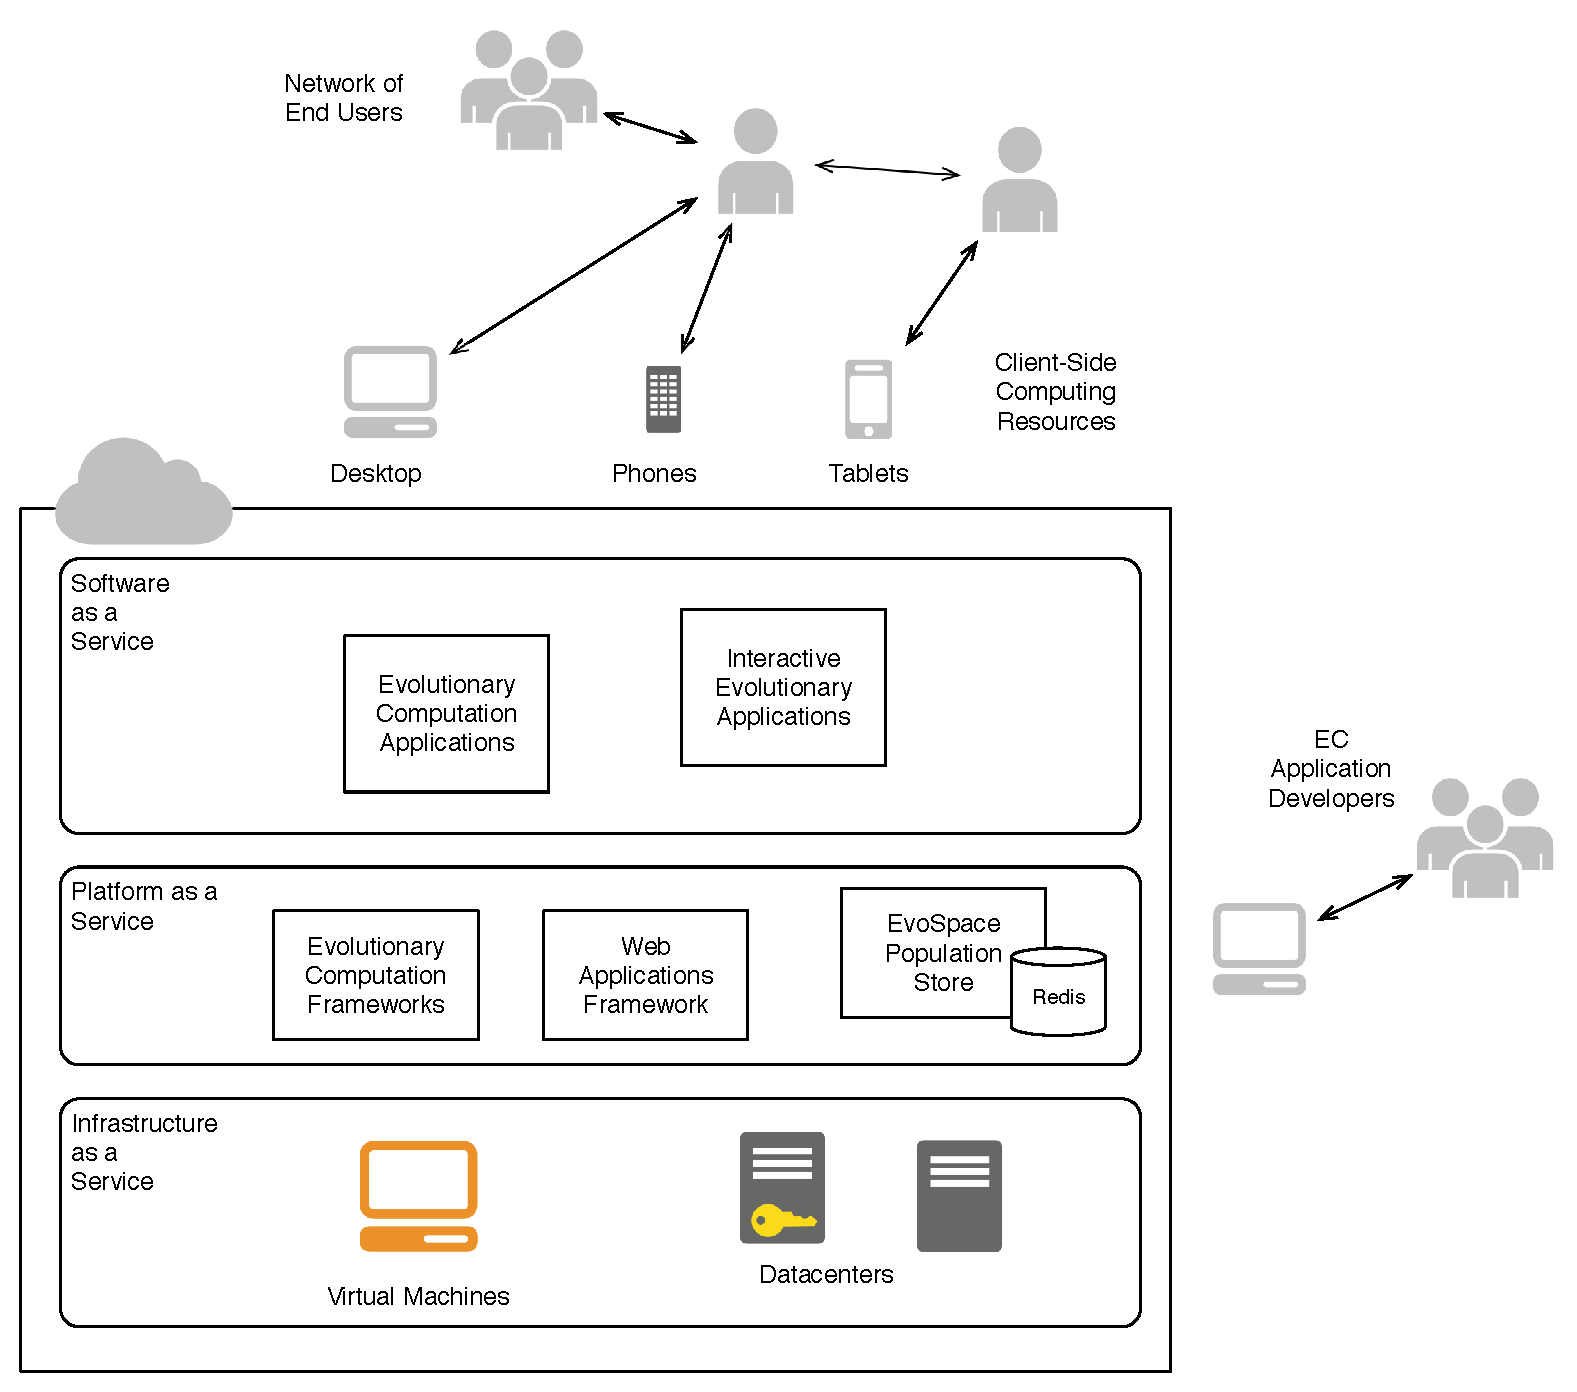
\includegraphics[width=12cm]{cloud2.eps}
    \caption{Conceptual diagram of the Cloud Computing Model and of how EvoSpace can fit within, using it as a PaaS or possible using it to develop a SaaS.}
    \label{fig:cloud} %this says that EvoSpace is basically a
                      %population store, is that correct? Then, what
                      %we are describing in this paper is something
                      %completely different and more wide-ranging - JJ 
\end{figure*}


\subsection{System Design}
Basically, EvoSpace consists of two main components. % You can't keep
                                % re-defining EvoSpace. Later on you
                                % say it's based on the tuple space
                                % model. And the graph above includes
                                % only one EvoSpace box: population
                                % store. 
First, the EvoSpace container object, which resides on a central server and stores the evolving population.
The second component consists of remote EvoWorkers, which are distributed processes that are executed on client machines connected to the server.
EvoWorkers execute the actual evolutionary process, while EvoSpace only serves as a population repository.
In summary, EvoWorkers extract a small subset of the population, and use it as
the initial population for a short evolutionary algorithm that is executed
locally on the client machine. Afterwards, the evolved population from each EvoWorker is returned and reinserted into the EvoSpace container.
The server-side ReInsert process is used to alleviate possible problems that might occur during the search, such when the EvoSpace container
is emptied or when connections are lost with connected EvoWorker clients.
Figure \ref{fig:evo} presents a graphical illustration of the main components and data-flow within EvoSpace.

\begin{figure*}[t]
    \centering
        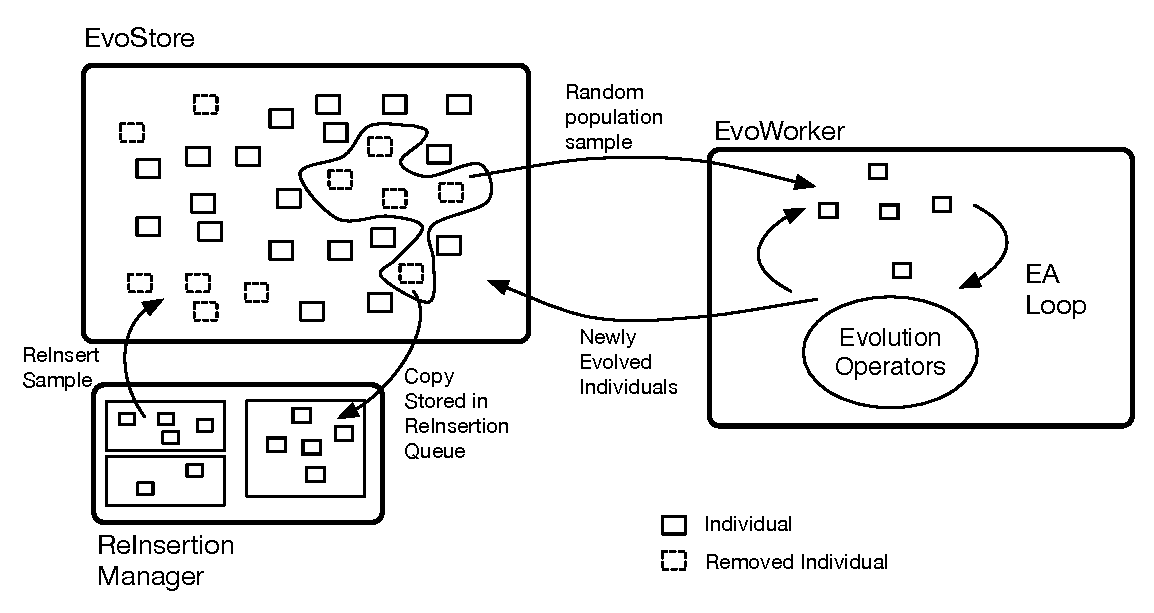
\includegraphics[width=12cm]{evospaceExample.eps}
    \caption{Main components and dataflow within EvoSpace.}
    \label{fig:evo}
\end{figure*}

% In all these sections there's a lot of description but very little
% fo the rationale behind them. Why did you do it this way? That
% applies to sections above and below - JJ
\subsubsection{The EvoSpace container}
\label{sss:container}
%This should be included in the Fig 1. Is it the same as the
%Population Store? In Fig. 2 EvoSpace is only the population store. 
EvoSpace is based on %based on? an implementation of? If it¡'s based
                     %on, what is the difference? 
 the tuple space model, an associatively addressed
%Wouldn't that be the "EvoSpace population store"? Isn't evospace the
%whole enchilada? - JJ
memory space shared by several processes. 
A tuple space can be described as a distributed shared memory (DSM) abstraction, organized as a \emph{bag} of tuples.
A tuple $t$ is the basic tuple space element, composed by one or more fields and corresponding values.
In this model, the basic operations that a process can perform is to
insert or withdraw tuples from the tuple space. % You could say here
                                % that's it's different from SofEA,
                                % since SofEA is an _array_ of tuples
                                % that can't be accessed randomly - JJ 

EvoSpace is composed by a set of objects $ES$ and a set of interface methods provided by a central server.
For an EA system, objects correspond to individuals.
Objects can be withdrawn, processed and replaced into $ES$ using a specified set of methods.
However, EvoSpace is different from other tuple space implementations in the sense that retrieving and reading objects from ES are random operations.
Individual objects are not of high interest when accessing $ES$.
Therefore, EvoSpace offers the following interface methods:
%El parrafo anterior se me hace confuso

\begin{itemize}
 \item \textbf{Read(n):} This method returns a random set $A$ of objects from $ES$, with $|A|=n$ and $A\subset ES$, if $n< |ES|$, the method returns $ES$ otherwise.

 \item \textbf{Take(n):} Returns a random set $A$, following the same logic used for $Read()$.
However, in this case a sequence of $Take()$ operations provide a temporal dimension to the dynamics of set $ES$.
We can define $ES_i$ as the set at the moment of the $i-th$ $Take()$ operation and $A_i$ as the output.
The contents of EvoSapce are then given by $ES_{i+1}= ES_i \setminus A_i$; i.e., the objets taken are effectively removed from $ES$.
The objects taken are also copied to a new set $S_i$ of \emph{sampled objects} and stored
within a temporary collection $\mathcal{S}$ on the server, implemented as a priority queue.
Sets $S_i \in \mathcal{S}$ can then be reinserted to $ES$ if necessary.

 \item \textbf{ReInsert(i):} This method is used to reinsert the subset of elements removed by the $i-th$ $Take()$ operation,
  such that the contents of EvoSpace are now $ES \cup S_i$ if $S_i \in \mathcal{S}$ and $ES$ is left unchanged otherwise.

 \item \textbf{Insert(A):} This method represents the union operation $ES \cup A$.

 \item \textbf{Replace(A,i):} Similar to $Add()$, however set $A$ should be understood as a replacement for
  some $S_i \in \mathcal{S}$, hence $|A| = |S_i|$, but the objects in $A$ can be different (evolved) objects from those in $S_i$.
  Moreover, if $S_i$ exists it is removed from $\mathcal{S}$.
  However, if $S_i$ does not exist this means that a $ReInsert(i)$ operation preceded it, this increases the size of $ES$.

 \item \textbf{Remove(A):} This method removes all of the objects in $A$ that are also in $ES$, in such a way that
  the contents of EvoSpace are now set to $ES \cup (A\cap ES)$.
\end{itemize}

\subsubsection{Individuals}
As stated above, objects in $ES$ represent individuals in an EA.
Explicitly, the objects in $ES$ are stored as \emph{dictionaries}, an abstract data type that represents a collection
of unique keys and values with a one to one association.
In this case, keys represent specific properties of each object and the values can be of different types, such as
numbers, strings, lists, tuples or other dictionaries.
In the current implementation, the objects in $ES$ are described by the following basic fields.
An \textbf{id} string that represents a unique identifier for each object.
A \textbf{chromosome} string, which depends on the EA and the representation used.
The \textbf{fitness} dictionary for each individual; allowing the system to store multiple fitness values for multi-objective or dynamic scenarios.
A \textbf{parents} dictionary with identifiers of the individual(s) from which it was produced.
Finally, a \textbf{GeneticOperator}  string that specifies the
operator that produced it. %Are you using this for something? Why do
                           %you need it - JJ ?


\subsubsection{The EvoSpace Server Processes}

%This is the key part of the system. Thoughts that went into it should
%be explicit. In CouchDB we didn't use reinsertion, for instance. Why
%do you do it here? Are you going to validate it in this paper? - JJ 
The EvoSpace architecture employs a client-server architecture with a shared memory container.
On the server side, a process called \textbf{EvoSpaceServer} is executed, which creates and activates a new EvoSpace
container object and waits for requests to execute interface methods; see Algorithm \ref{alg:evoserver}.
Additionally, on the server two more processes are executed, these are: \textbf{InitializePopulation} and \textbf{ReInsertionManager} ;
see algorithms \ref{alg:population} and \ref{alg:remanager}.
\textbf{InitializePopulation} is executed once, its goal is obvious, initialize the population by adding $popsize$ random
individuals. The function that creates new individuals depends on the problem and representation used.
\textbf{ReInsertionManager} is used as a failsafe process that periodically checks (every $wt$ seconds) if the size of the population in $ES$
falls below a certain threshold or if the time after the last $ReInsert()$ is greater than $next_r$.
If any of these conditions are satisfied, then $rn$ subsets $S_i \in \mathcal{S}$ are reinserted into ES using the $ReInsert()$ method.
Moreover, the \textbf{ReInsertionManager} makes a $ReInsert(i)$ call when $EvoWorker_i$ (see below) looses a connection with the server,
thus recovering the population sample.
%Finally, \textbf{EvolutionManager} periodically checks if a termination condition is satisfied, which is checked by the $isOver()$ method.
%This method can be implemented according to the needs of the evolutionary search.
%For instance, $isOver()$ can check if an optimal solution is found or if a maximum number of function evaluations have been performed.
%No hay EvolutionManager cada worker consulta al EvoSpace
\begin{algorithm}[t]
\label{alg:evoserver}
\caption{The server-side \textbf{EvoSpaceServer} process.}
\begin{algorithmic}
\STATE $EvoSpace$ $\leftarrow$ new EvoSpace
\STATE $EvoSpace.active$ $\leftarrow$ true
\WHILE{$EvoSpace.active$}
\STATE read method
\RETURN $EvoSpace.method()$
\ENDWHILE
\end{algorithmic}
\end{algorithm}


\begin{algorithm}[t]
\label{alg:population}
\caption{The server-side \textbf{InitializePopulation} process.}
\begin{algorithmic}
\REQUIRE $EvoSpace \leftarrow$ Reference to an Evospace Server
\REQUIRE $popsize \leftarrow$ Number of individuals
\STATE $j \leftarrow 0$
\FOR{$j < popsize$}
\STATE $ind$ $\leftarrow$ new individual() \COMMENT{Problem dependent}
\STATE $EvoSpace.ES.Add(i)$
\STATE j++
\ENDFOR
\end{algorithmic}
\end{algorithm}

\begin{algorithm}[t]
\label{alg:remanager}
\caption{The server-side \textbf{ReInsertionManager} process.}
\begin{algorithmic}
\REQUIRE $ri \leftarrow$ re-insertion interval
\REQUIRE $min \leftarrow$ population size threshold
\REQUIRE $rn \leftarrow$ number of samples to re-insert
\REQUIRE $EvoSpace \leftarrow$ Reference to an Evospace Server
\REQUIRE $wt \leftarrow$ wait interval
\STATE $next_r \leftarrow +ri$
\WHILE{$EvoSpace.active$}
\IF{$|EvoSpace.ES| \leq min$ OR $currentTime \geq next_r$}
\STATE $EvoSpace.RespawnOld(rn)$
\STATE $next_r \leftarrow currentTime + ri$
\ENDIF
\STATE $wait(wt)$
\ENDWHILE
\end{algorithmic}
\end{algorithm}



\subsubsection{The EvoSpace Clients: EvoWorkers}
The second component of the proposed model are the processes executed on client machines, referred to as \textbf{EvoWorkers}, see Algorithm \ref{alg:worker}.
Each client loads a process that executes the main code of the EA.
The \textbf{EvoWorker} process is straightforward, it requests a set of objects $A_i$ from the $ES$ container.
Afterwards, the $Evolve()$ function is called where the actual evolutionary cycle is performed.
In this scenario, $A_i$ can be seen as a local population on which evolution is carried out for $g$ generations.
The result of this evolution is then returned and reinserted into $ES$, then the EvoWorker can request a new set from $ES$ and repeat the process.
Otherwise, each EvoWorker could specialize on a particular part of the evolutionary process, such as selection, evaluation or genetic variation;
an approach not taken in the present work.
%We could add a comment indicating that even a person could do part of the job, for instance assigning fitness in an interactive EA. (Mario)

\begin{algorithm}[t]
\label{alg:worker}
\caption{The client-side \textbf{EvoWorker} process.}
\begin{algorithmic}
\REQUIRE $EvoSpace \leftarrow$ Reference to an Evospace Server
\REQUIRE $n \leftarrow$ sample size
\REQUIRE $rt \leftarrow$ retry time
\REQUIRE $g \leftarrow$ number of generations

\WHILE{EvoSpace.ES.active}
\STATE $S_i \leftarrow ES.Take(n)$
\IF{$A_i$ \textbf{is not} null}
\STATE $Evolve(A,g)$
\STATE $EvoSpace.ES.Replace(A_i)$
\ELSE
\STATE $wait(rt)$
\ENDIF
\ENDWHILE
\end{algorithmic}
\end{algorithm}

\subsubsection{Implementation}
Figure~\ref{fig:evospace} shows a schematic diagram of the proposed architecture and the corresponding information flow with implementation details.
Individuals are stored in-memory, using the Redis key-value
database. 
Redis was chosen over a SQL-based management system, or other non-SQL
alternatives, because it provides a hash based implementation of sets
and queues which are natural data structures for the EvoSpace
bag-of-tuples models mentioned in Sec \ref{sss:container}. 
model. For example, selecting a random key from a set has a complexity
of O(1). The logic of EvoSpace is implemented as a Python module
exposed as a  
JSON-RPC Service using Cherrypy and Django HTTP frameworks.
The EvoSpace service % service? System? Implementation? You should
                     % _really_ provide a conceptual model of
                     % everything - JJ 
can interact with any language supporting {\tt json-rpc} or Ajax requests. The EvoSpace module and EvoWorker implementations in JavaScript and Python are available with a Simplified BSD License from \url{http://github.com/mariosky/EvoSpace}.

\begin{figure*}[t]
    \centering
        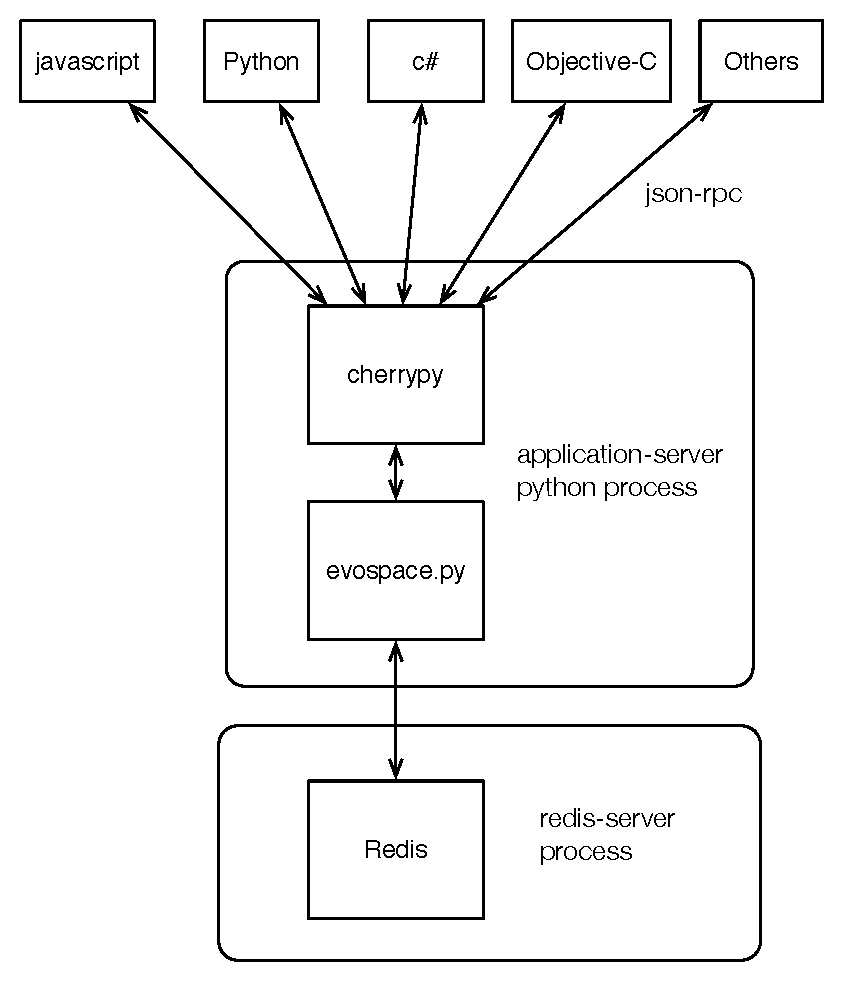
\includegraphics[width=8cm]{evospace.eps}
    \caption{Evospace Implementation architecture } %EvoSpace the
                                %whole enchilada? EvoSpace the
                                %population store? Why implementation
                                %in Capitals? - JJ
    \label{fig:evospace}
\end{figure*}

As EvoSpace is only the population store, EvoWorkers must implement the genetic operators of a particular EA.
As stated earlier, our objective is to let researchers use common tools as in their local setting.
Given that EvoSpace is implemented as a Python module, a simple way to implement EvoWorkers is using a basic non-distributed GA found in the DEAP (Distributed Evolutionary Algorithms in Python) library \cite{DEAP_JMLR2012}.  Three methods were added to the local DEAP algorithm: $getSample()$ and  $putSample()$; and  another for the  initialization of the population using DEAP´s own methods.
For instance, to generate the initial population DEAP's initialize() method  is called and the generated population is sent to EvoSpace, then for each generation $getSample()$ is called, the received sample is used to create a DEAP population which is then evolved for a number of generations. Finally the DEAP population is converted to a JSON object and is returned to EvoSpace calling the $putSample()$ method.   

%% TO DO: Write a more detailed explanation than above (Mario). 

\subsection{EvoSpace on the Cloud}
This section describes how EvoSpace can be configured to run on the Cloud using Heroku and PiCloud; a schematic view of the cloud architecture is shown in figure~\ref{herokuPiCloud}.

\begin{figure}[t]
\centering
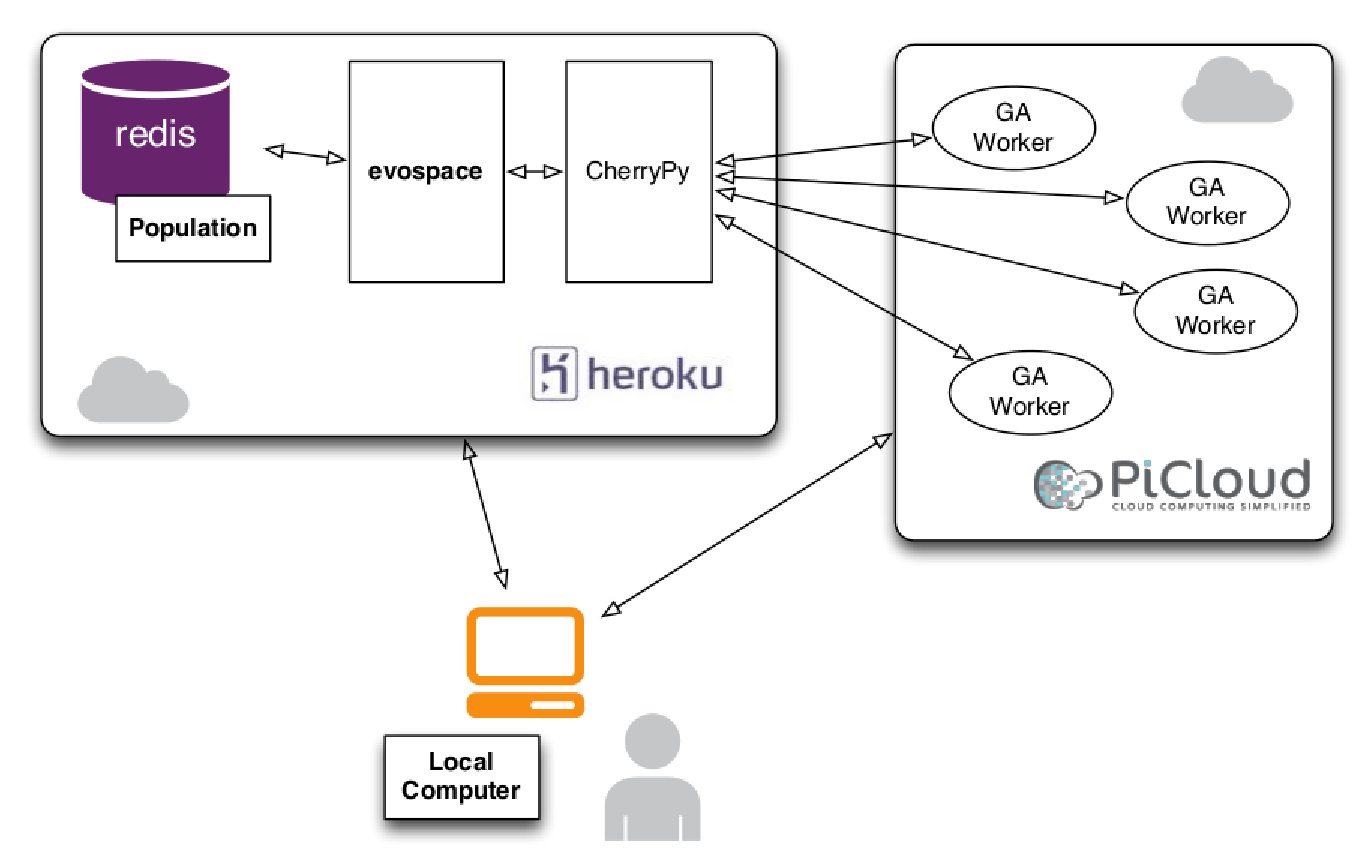
\includegraphics[width=3.2in]{herokuPiCloud.eps}
\caption{EvoSpace cloud-based architecture.}
\label{herokuPiCloud}
\end{figure}


\subsection{Evospace as a Heroku Application}

Heroku (\url{http://heroku.com}) is a multi-language PaaS, supporting among others Ruby, Python and Java applications. The basic unit of composition on
Heroku is a lightweight container running a single user-specified
process. These containers, which they call {\em dynos}, can include web
(only these can receive {\tt HTTP} requests) and worker processes
(for instance processes used for database backups or task queues).
These  process types are the prototypes from which one or more dynos 
can be instantiated; if the number of requests to the server increases then 
more instances can be assigned on-the-fly. In our case, our CherryPy 
web application server runs in one web process, when the number 
of workers was increased we added more dynos (instances) of the 
CherryPy process. This model is very different from a Virtual Private Server (VPS) where users pay for the whole server; in a process based model, users pay only for the processes they need; being a {\em freemium} model means also that, if a minimum level of resources is not exceeded, it can be used for
free. 
Once deployed the web process can be scaled up by assigning more dynos;
in our case and in the more demanding experiments, the web process was scaled to 20 dynos. Instructions and code for deployment is available at \url{http://www.evospace.org/software.html} 


\subsection{Evoworkers as PiCloud Jobs}
PiCloud is a PaaS, with deep Python integration; 
using a library, Python functions are transparently uploaded to PiCLoud's 
servers as units of computational work they call \emph{jobs}. 
Each job is added to a queue, and when there is a core available, 
the job is assigned to it. Both Heroku and PiCloud 
platforms are deployed on top of Amazon Web Services (AWS) 
infrastructure in the US-EAST Region. This ensures minimal 
latency and a high bandwidth communication between the services, 
and there is no charge for data transfer costs between both services.
For the experiments type c1 and c2 Real Time workers where used.  
The code for the EvoWorkers implementation and experiment data is publicly available from a Github repository \url{https://github.com/mariosky/evoPar2014}. 
% \url{http://goo.gl/92tMFw}. % Github tiene su
                                % propio acortador, pero también
                                % tienes que anonimizarlo - JJ 
The following sections present an experimental evaluation of EvoSpace using standard benchmark problems for GAs.
In particular, EvoSpace is first evaluated based on performance and efficiency, compared to a canonical GA, this is done
in Section \ref{sec:exp1}.
Afterwards, specific issues with PEA algorithms are discussed and experimentally evaluated in Section \ref{sec:overcome},
that illustrate how potential shortcomings are avoided with the EvoSpace framework.


\section{Experiments and Results}
\label{sec:exp1}
This section presents an experimental evaluation of EvoSpace using two well-known benchmarks for GAs;
the K-trap problem \cite{trap} and the P-Peaks function
\cite{Jong:PS97}. %To prove what? Validate the approach? Check
                  %performance? Scalability? Both? - JJ

\subsection{Experiment A: K-trap Function}
This problem presents a multi-modal and deceptive fitness landscape.
Table \ref{tab:exp} summarizes the different experimental configurations tested in this work, based on the $K$ value, number of EvoWorkers, the sample size taken by each worker and the chromosome length used in each K-trap problem. The number of individuals in the EvoSpace repository is set to 1024 for 4-trap experiments and to 4096 for 5-trap.
Moreover, Table \ref{tab:exp2} summarizes the shared parameters and algorithmic configuration.
The maximum number of samples that each EvoWorker can take from EvoSpace is 1000.
For comparison, a standard GA is applied to each benchmark problem.
For the 4-trap problem, the maximum number of generations is 4000, for the 5-trap problem it is 1000,
this bounds the number of function evaluations based on the maximum number of samples taken from all of the EvoSpace runs.
In total, $50$ runs were performed of each experimental configuration.


\begin{figure*}[t]
    \centering
    \subfigure[Evolution of Fitness]
    {
       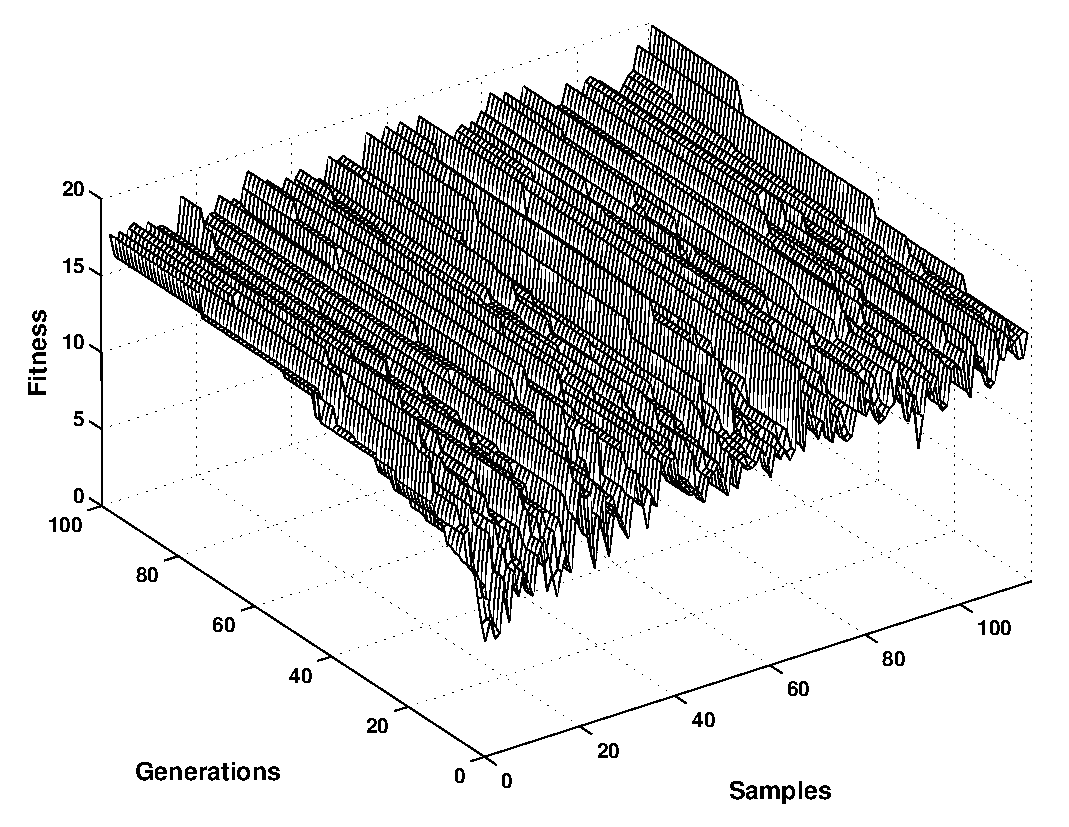
\includegraphics[width=5.5cm]{Plot-Surface-Best-Run0-k5w4s64.eps}
       %\includegraphics[width=5cm]{Plot-Individuals-Eval-k4w32s32.eps}

    }
    \subfigure[Evaluated]
    {
        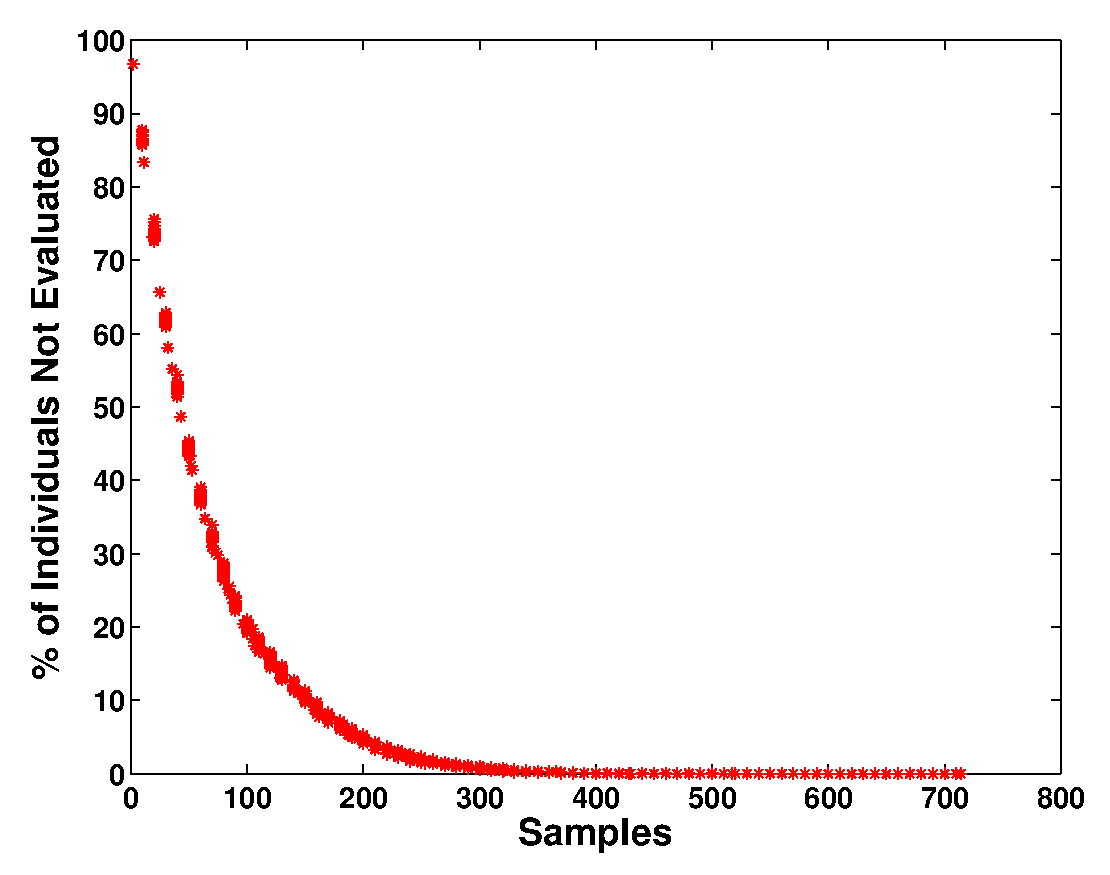
\includegraphics[width=5.5cm]{Plot-Individuals-Eval-k5w4s64.eps}
    }
    \\
    \subfigure[Experiment K]
    {
        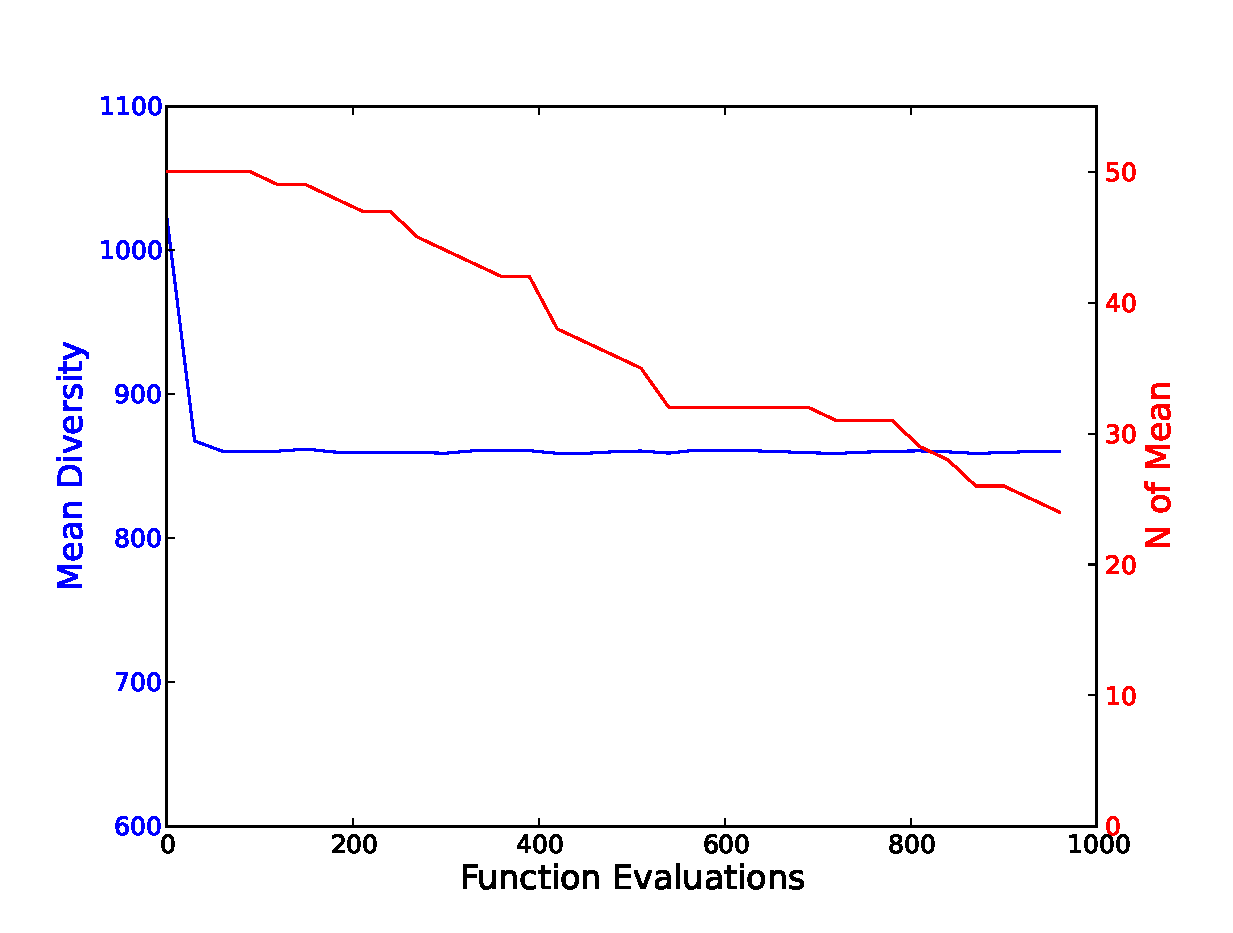
\includegraphics[width=5.5cm]{DivMeanEvoSameScale.eps}
    }
    \subfigure[Standard GA]
    {
        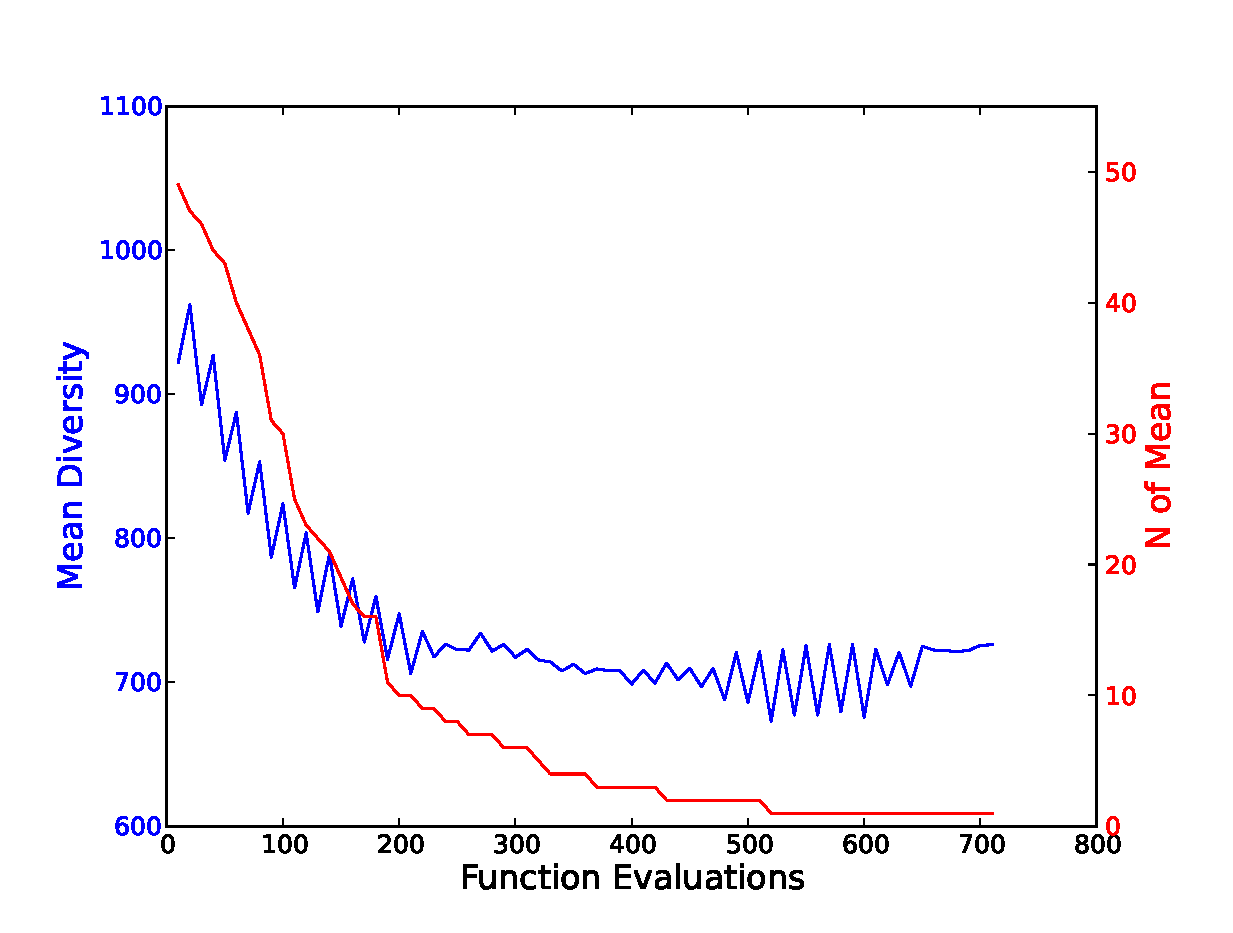
\includegraphics[width=5.5cm]{DivMeanGASameScale.eps}
    }
    \caption{
    (a) Evolution of fitness for a run of experiment K; the plot shows how fitness evolves for each sample taken by the EvoWorkers.
    (b) Scatter plot, considering all runs, of the percentage of non-evaluated individuals from experiment K.
    (c) Evolution of diversity in EvoSpace for experiment K.
    Plots c-d are double y-axis plots, showing the mean diversity over all runs (dark line) and the number of runs $N$ used to compute the mean.
    (d) Evolution of diversity for the basic GA on the 5-trap problem.}
    \label{fig:others}
\end{figure*}

Figure \ref{fig:others}a depicts how fitness evolves over all of the samples taken from EvoSpace.
This figure shows the evolution of best-fitness for a single run of experiment K in Table \ref{tab:exp};
the analysis focuses on a single run instead of the mean of all runs to emphasize the local dynamics of the evolutionary process.
The plot shows how fitness evolved on each EvoWorker that participated in the search.
Evolution of fitness is organized based on the two temporal axis of the horizontal plane,
one corresponds with the sample number, independent of which EvoWorker took the sample, and the other corresponds
to the generations of the local evolutionary process executed on the EvoWorker.
In other words, these plots provide a collective view of the evolutionary process from the perspective of all EvoWorkers.
Since the global optimum is a fitness value of 10, we can see that the evolution on the last sample taken from EvoSpace reaches the global optimum.
%and after this no more samples are taken since the search is halted at that moment.
The overall performance of EvoSpace is summarized in Table \ref{tab:found}, which shows the total number of runs, out of $50$,
that found the global optima.
EvoSpace outperforms the standard GA on both functions, with a substantial increase in the number of optima found.

\begin{table}[t]
\caption{Different experimental configurations used to test the
  performance of EvoSpace.} %Why these? What do you want to evaluate?
                            %Is it complete? 
\centering
\tiny
\begin{tabular}{|l||c|c|c|c|c|c|c|c|c|c|c|c|c|c|c|}
   \hline
             \textbf{Experiment} 	& A & B & C & D & E & F & G & H & I & J & K & L & M & N & O \\

   \hline
               \textbf{K-trap}   	& 4  & 4  & 4  & 4  & 4  & 4  & 4  & 4  & 4 & 5 & 5 & 5 & 5 & 5 & 5 \\
			   \textbf{EvoWorkers}  & 1  & 1  & 4  & 4  & 8  & 8  & 16 & 16 & 32 & 1 & 4 & 8 & 16 & 32 & 40 \\
			   \textbf{Sample size} & 32 & 64 & 32 & 64 & 32 & 64 & 32 & 64 & 32 & 64 & 64 & 64 & 64 & 64 & 64 \\
			   \textbf{Chromosome length} & 40 & 40 & 40 & 40 & 40 & 40 & 40 & 40 & 40 & 50 & 50 & 50 & 50 & 50 & 50 \\
   \hline
\end{tabular}
\label{tab:exp}
\end{table}


\begin{table}[t]
\caption{Parameters and algorithm configurations for all experiments.}
\centering
\begin{tabular}{|c||c|c|c|c|}
   \hline
                       & Maximum Function         &                    &                  & Generations per \\
   \textbf{Parameter}  & Evaluations              & Crossover (Prob.)  & Mutation (Prob.) & EvoWorker        \\

	\hline
   \textbf{Value}     &	100 Gens per worker &	Single point (1) &	Point  (0.06)   & 100    \\
   \hline

\end{tabular}
\label{tab:exp2}
\end{table}


\begin{table}[t]
\caption{Different experimental configurations used to test the performance of EvoSpace.
GA-K are the baseline GA results for the 4-trap and 5-trap functions respectively.}
\centering
\tiny
\begin{tabular}{|l||c|c|c|c|c|c|c|c|c|c|c|c|c|c|c|c|c|}
   \hline
             \textbf{Experiment} & A & B & C & D & E & F & G & H & I & J & K & L & M & N & O & GA-4 & GA-5 \\

   \hline
        \textbf{Optima found}   & 48 & 50 & 50 & 49 & 49 & 50 & 48 & 50 & 50 & 50 & 50 & 50 & 50 & 50 & 50 & 34 & 29 \\

   \hline
\end{tabular}
\label{tab:found}
\end{table}

\begin{figure*}[t]
    \centering
    \subfigure[]
    {
        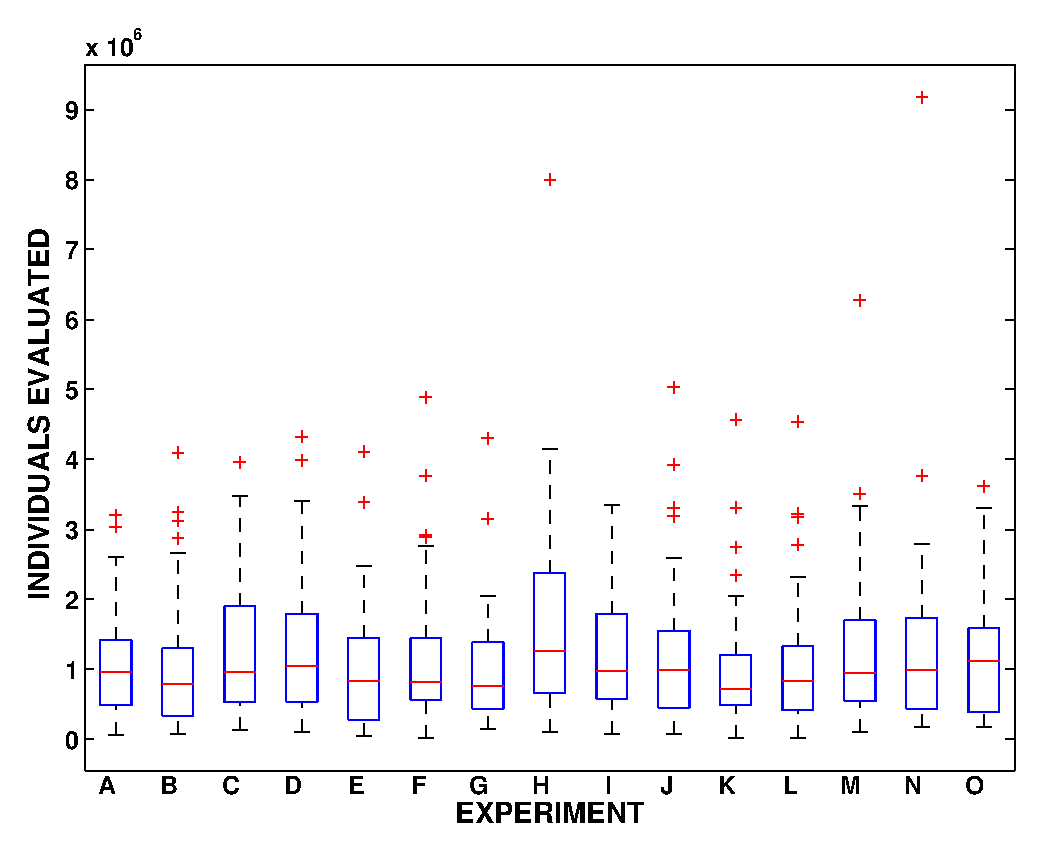
\includegraphics[width=5.5cm]{Evaluados.eps}
    }
    \subfigure[]
    {
        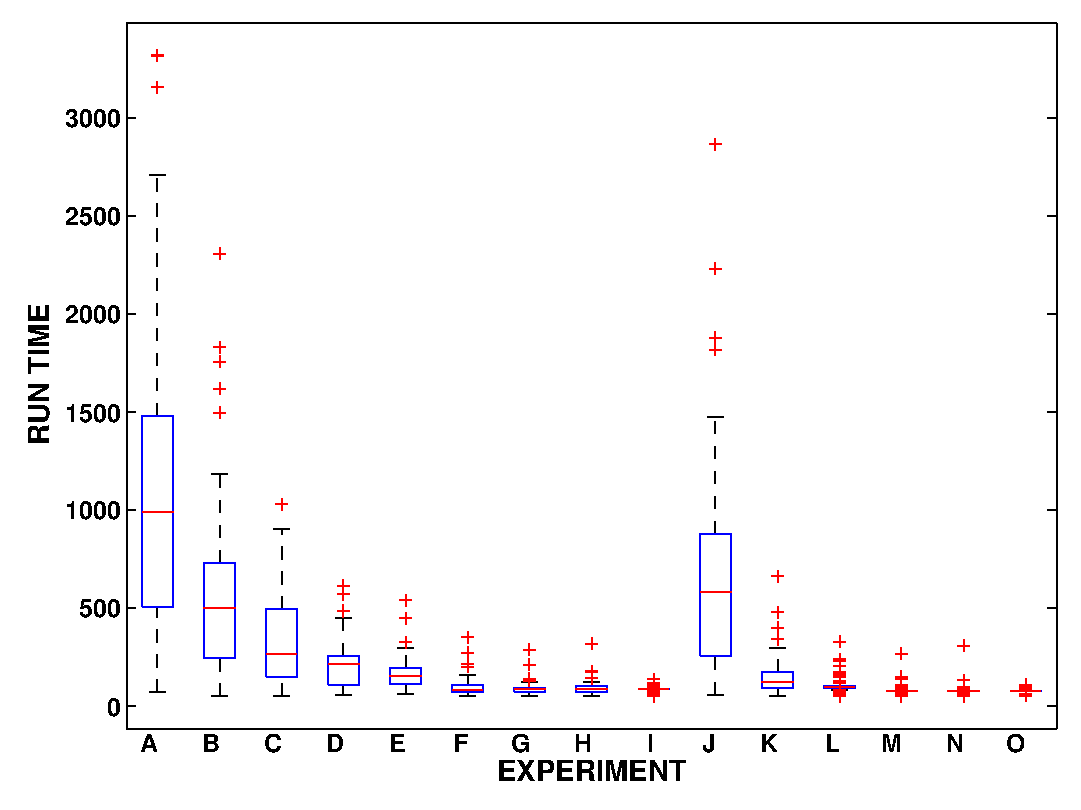
\includegraphics[width=5.5cm]{TimeBox.eps}
    }
    \caption{
    (a) Number of evaluated individuals.
    (b) Total run-time.}
    \label{fig:effort}
\end{figure*}

Since every EvoWorker takes a random sample of individuals, one concern might be that some individuals of the initial population might
not be chosen and evaluated wasting valuable genetic material.
However, Figure \ref{fig:others}b shows that the percentage of not evaluated individuals within EvoSpace quickly decreases as more samples are taken.
Another interesting question is how the EvoSpace search impacts diversity, here given by the sum of the pairwise Hamming distances
of all individuals within the population \cite{diversity}.
Figure \ref{fig:others}c shows how diversity evolves for experiment K, and
Figure \ref{fig:others}d shows the same for the basic GA\footnote{The time scale is given by
the number of individuals evaluated, increments correspond to the number of individuals evaluated in 10 samples.}
These plots show how the standard GA has a problem maintaining diversity, which leads to its poor performance shown in Table \ref{tab:found}.
On the other hand, EvoSpace maintains a more diverse population which leads to a better exploration of the search space and more successful runs.

Finally, a comparison of the computational effort required in each experiment is given in
Figure \ref{fig:effort}, which shows boxplots of all runs in each experiment.
Figure \ref{fig:effort}a plots the total number of individuals evaluated in each run, which is similar in all experiments;
while Figure \ref{fig:effort}b compares the total run time in seconds.
Figures show that run time is significantly reduced as the number of EvoWorkers increases.



\subsubsection{Experiment B: P-Peaks}
% Why this second experiment? Do you want to prove something you
% haven't before?  - JJ 

The P-Peaks problem was chosen because the problem and consequently the computing resources needed for the search can be appropriately scaled.
Proposed by De Jong et al. in \cite{Jong:PS97}, as a generalization of the version in \cite{Jong:1990}, a
P-Peaks instance is created by generating a set of P random N-bit
strings, which represent the location of the P peaks in the space. To
evaluate an arbitrary bit string \begin{math} \mathbf{x} \end{math}
first locate the nearest peak (in Hamming space). Then the fitness of
the bit string is the number of bits the string has in common with
that nearest peak, divided by N. The optimum fitness for an individual
is 1, and is computed by

\begin{equation}
f_{P-PEAKS}(\mathbf{x})=\frac{1}{N} \overset{P}{\max_{i=1}} \{N-hamming(\mathbf{x},Peak_i)   \} \ .
\end{equation}

A large number of peaks induces a time-consuming search,
since evaluating every string is computationally expensive; this is
convenient since in order to justify a distributed EA fitness computation has to be significantly larger than the associated
network latency (otherwise, it would always be faster to have a single-processor version).
For this work, the experiment is setup with $P = 256$ peaks and $N = 512$ bits, a configuration that requires considerable computational time for
fitness evaluation, and 30 runs are performed.
Regarding algorithm parameters these are summarized in Table \ref{tab:paramse}.

\begin{table}[t]
\renewcommand{\arraystretch}{1.3}
\caption{GA and EvoWorker parameters for experiments.}
\label{tab:paramse}
\centering
\begin{tabular}{|l||c|}
\hline
\multicolumn{2}{|c|}{GA Parameters} \\
\hline
Tournament size & 4 \\
Crossover rate & 0.85  \\
Population Size & 512 \\
Mutation probability & 0.5 \\
Independent bit flip probability  & 0.02 \\
\hline
\multicolumn{2}{|c|}{EvoWorker Parameters} \\
\hline
Sample Size & 16 \\
Generations & 128 \\
\hline
\multicolumn{2}{|c|}{Variable Parameters} \\
\hline
PiCloud Worker Type & Realtime, Standard \\
Number of Workers & 2,4,8,16,28 \\
Number of Executions & 30 \\
\hline

\end{tabular}
\end{table}

As a baseline execution, the experiment was also conducted in a local computer. The specifications for the local computer are as follows, a
2.2 Ghz Intel Core i7 processor, 16 GB of 1333 DDR3 memory, and Mac OS
X 10.7.5 operating system. All the experiments were executed in a Python
interpreter (version 2.7.2) for 64-bit architectures. 

In this setting, the problem required considerable computational time: each run took an average of 1567.36 seconds to find the optimal solution (see table~\ref{local}).
The execution used a single core in the computer and CPU activity remained low for the whole length of the experiment. On the other hand, the parallel execution time was significantly lower even when only two workers were used,
clocking at less than 180s even in the worst cases.

\begin{table}[t]
\renewcommand{\arraystretch}{1.3}
\caption{Average Times and Evaluations of 30 executions in a local computer.}
\label{local}
\centering
\begin{tabular}{|c|c|}
\hline
Average time in seconds & Average number of evaluations \\
\hline
1567.36 & 100690.5  \\
\hline
\end{tabular}
\end{table}

Average times for the configuration using Realtime cores in PiCloud,
are presented in Figure~\ref{fig:plot_time_real}. It can be seen that
incrementing the number of workers reduced the time to solution, but only up to 16 workers. With 28 workers time to solution did not improve. This is
related to the increase in the number of evaluations needed to find
the optima, which is shown in Figure~\ref{fig:plot_evals_real}.
This figure shows that the number of evaluations needed to find the
solution increases as more workers are used. This behavior has an
impact on the time to solution, because each evaluation (as stated
earlier), is computationally expensive. From 2 to 8 workers the number
of evaluations remains less than in the baseline GA, but from that point on
the number is higher. A possible reason for this is that as
the number of workers increases, the number of individuals that remain
in the population waiting to be replaced decreases. As there are fewer
individuals in the population the probability of taking the same individuals
when replacing a sample is increased. This problem is also reported
by Merelo et al. in  \cite{sofea:naco}, where they present a PEA architecture with heterogeneous workers.

For other problems where the evaluation of individuals is not very
demanding, the added cost of communication between EvoSpace and EvoWorkers can become a concern.
In these experiments this cost is negligible, Figure~\ref{plot_ges} shows boxplots of the time required two perform the
three main methods on the EvoWorkers from 30 runs of the 28 Realtime workers experiment.


\begin{figure*}[t]
    \centering
    \subfigure[Time to solution]
    {
        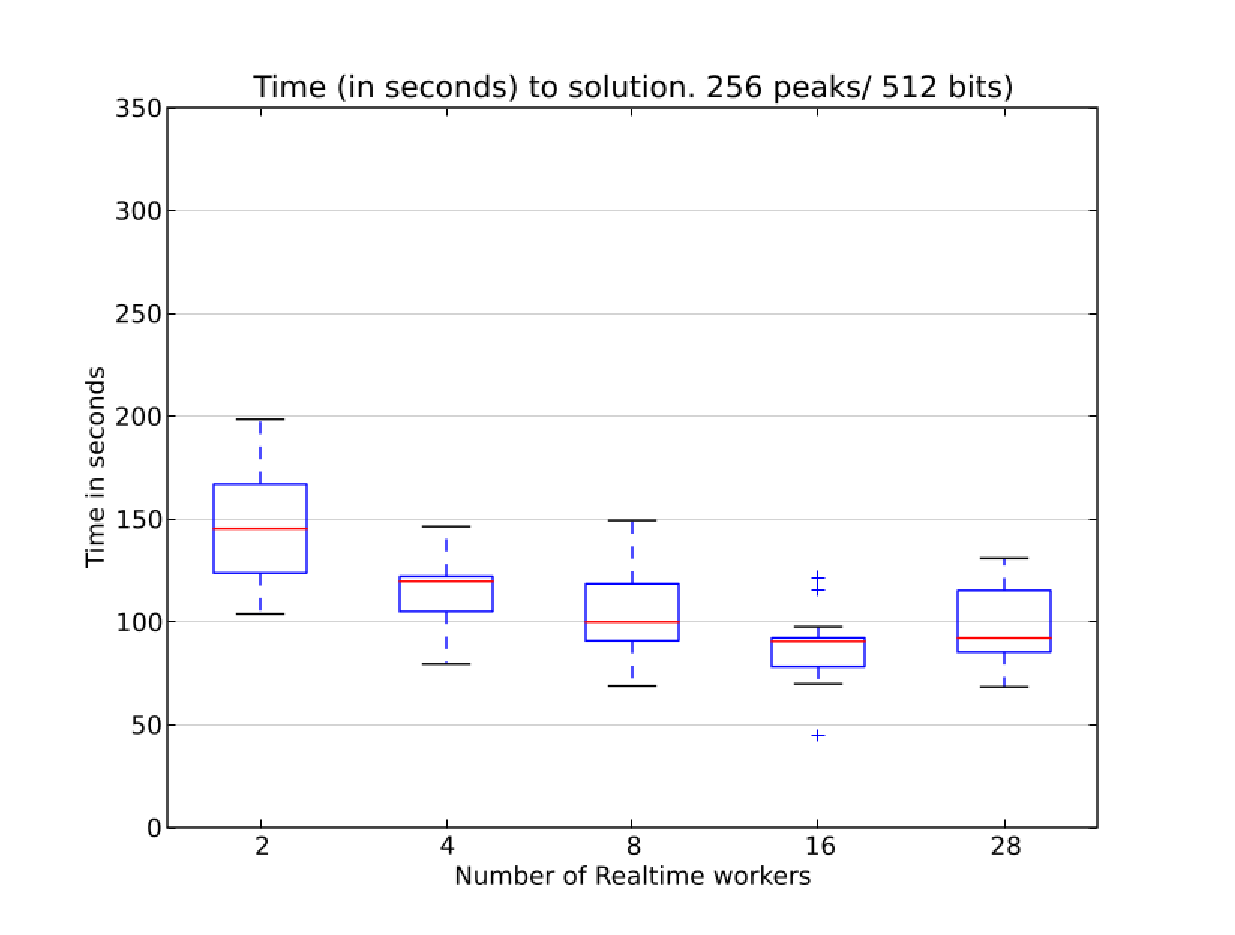
\includegraphics[width=5.5cm]{plot_time_realtime.eps}
        \label{fig:plot_time_real}
    }
    \subfigure[Number of Evaluations]
    {
        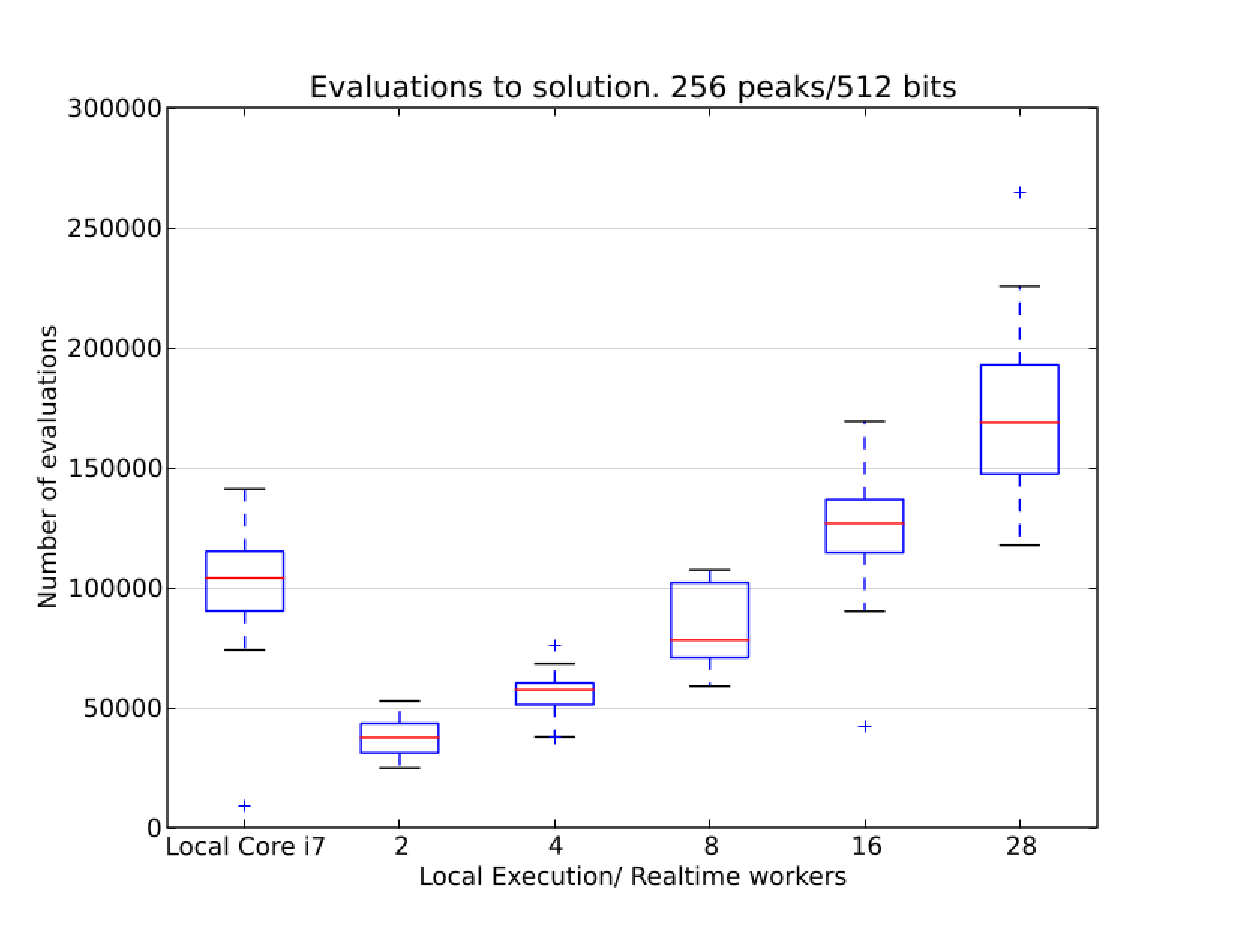
\includegraphics[width=5.5cm]{plot_evals_realtime.eps}
        \label{fig:plot_evals_real}
    }\\
        \subfigure[Worker Costs]
    {
        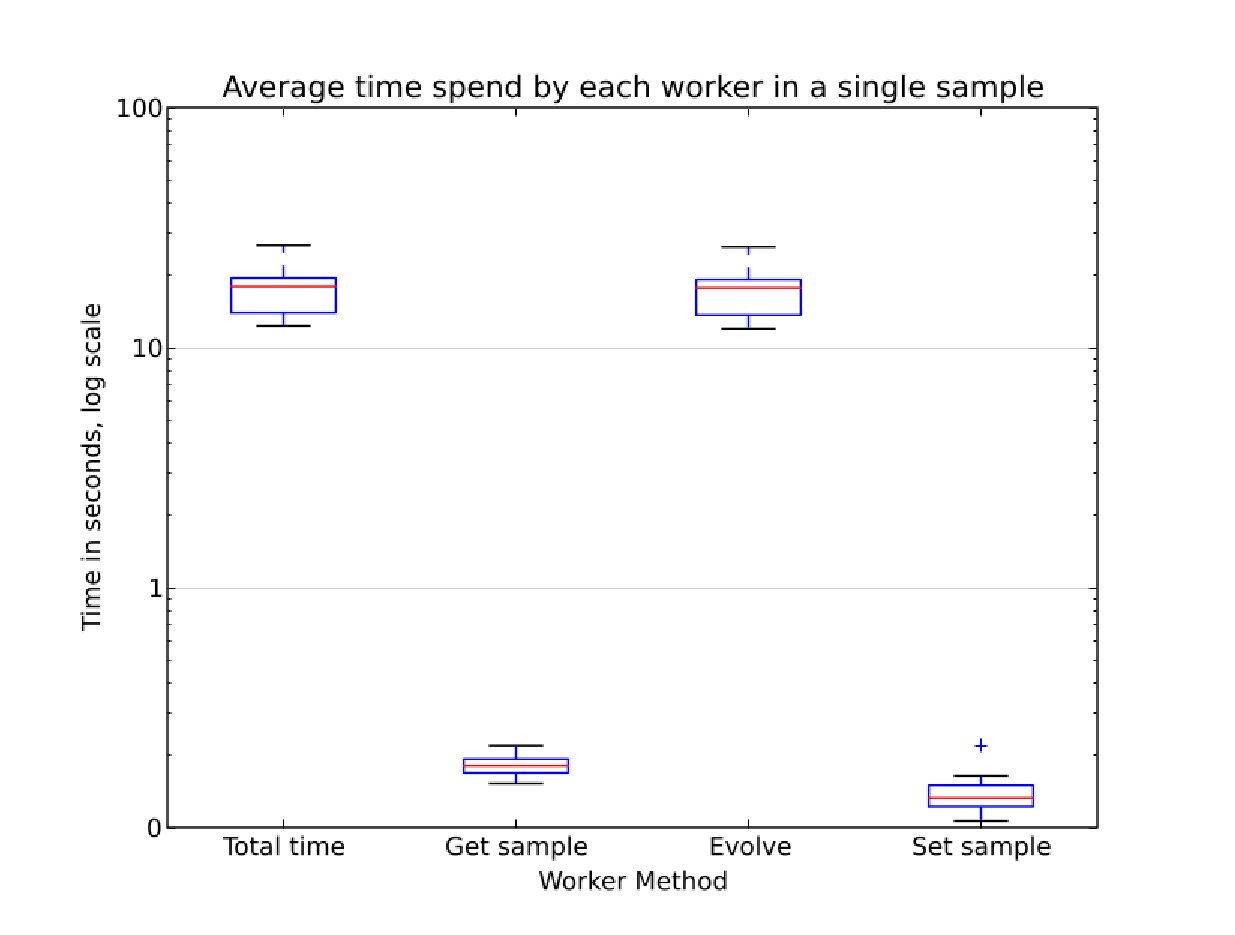
\includegraphics[width=5.5cm]{plot_ges.eps}
        \label{plot_ges}
    }
    \caption{
    (a) Time required to solution.
    (b) Number of evaluations to solution. (c) Time of worker's methods, GetSample(), Evolve(), PutSample().}
    \label{fig:effort_real_time}
\end{figure*}


%\subsection{Discussion}


\section{Overcoming Problems and Limitations}
\label{sec:overcome}
The previous section showed how EvoSpace can be used to implement a distributed and asynchronous EA, with strong results on two benchmark tests.
However, there are possible downsides to using a PEA such as EvoSpace, these include low bandwidth, abandoned work, system security and privacy, all of which are important issues. However, in what follows we focus on two critical issues, lost work due to the unreliable EvoWorkers,
and algorithm parametrization, a common issue with almost all EAs that is severely amplified in a PEA approach.

\subsection{Unreliable Workers}
In this section, the effect of node unavailability in an EvoSpace EA is assessed.
The EvoSpace model contrasts with the use of a global queue of tasks and implementations
of map-reduce algorithms, such as in \cite{fazenda2012}, with several benefits relevant to
concurrency control and workload distribution. 
For instance, leaving a copy of the individual in the population server
free to be pulled by other EvoWorkers will result in redundant work and this
could be costly if the task at hand is time consuming. Moreover, EvoWorkers are expected
to be unreliable, since they can loose a connection or could simply shut down or be removed from the client machine.
When an EvoWorker is lost, so are the individuals pulled from the population store.
Depending on the type of algorithm that is executed, the loss of these samples could have a high performance cost.
As stated before, to address this problem, EvoSpace uses a simple reinsertion algorithm that also prevents
the starvation of the population pool. Other pool based algorithms normally use
a random insertion technique, but this might negatively impact the search process.

\begin{figure*}[htp]
    \centering
    \subfigure[]
    {
        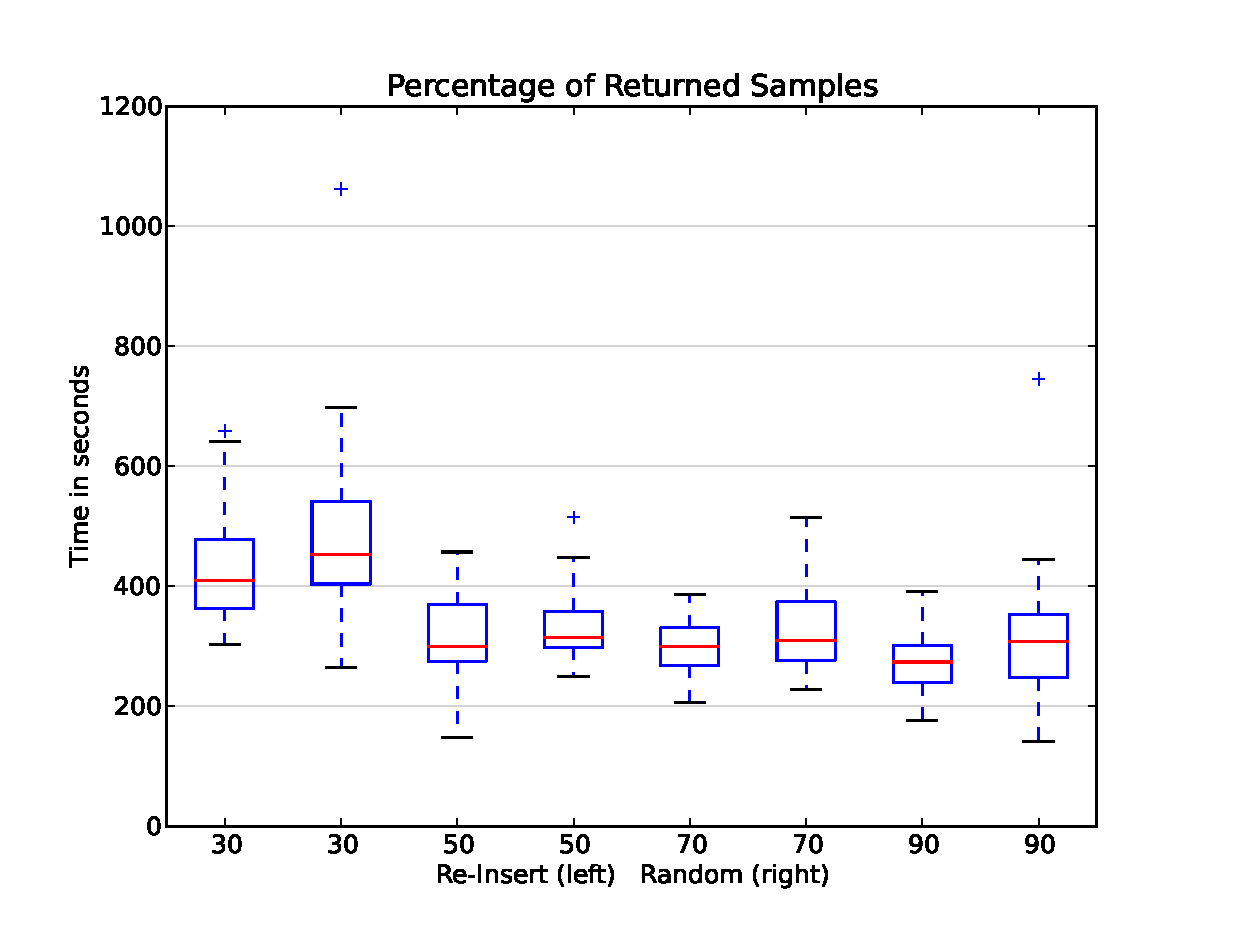
\includegraphics[width=5.5cm]{plot_time_CRS_w4.eps}
        \label{fig:plot_time_ri_w4}
    }
    \subfigure[]
    {
        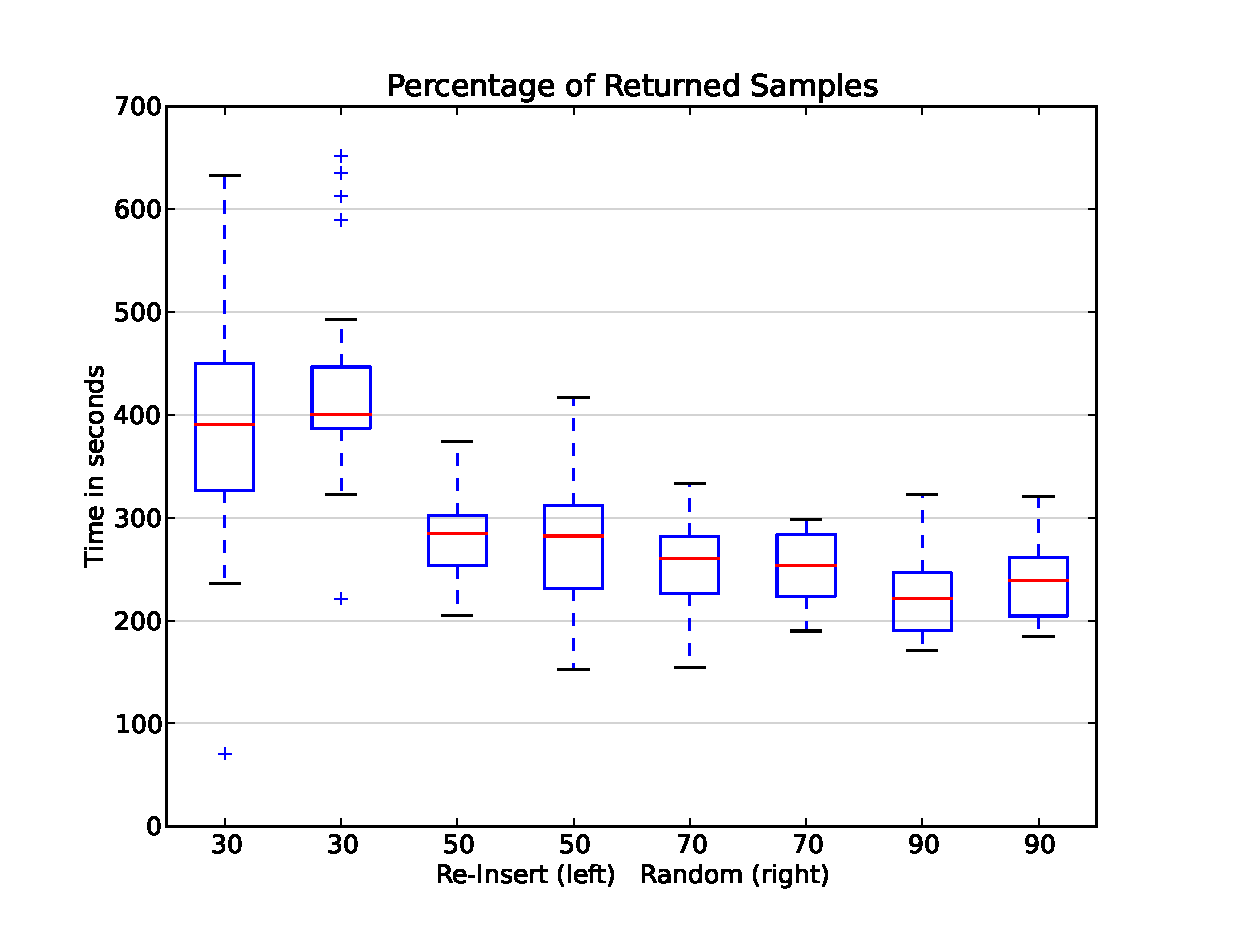
\includegraphics[width=5.5cm]{plot_time_CRS_w8.eps}
        \label{fig:plot_time_ri_w8}
    }
    \subfigure[]
    {
        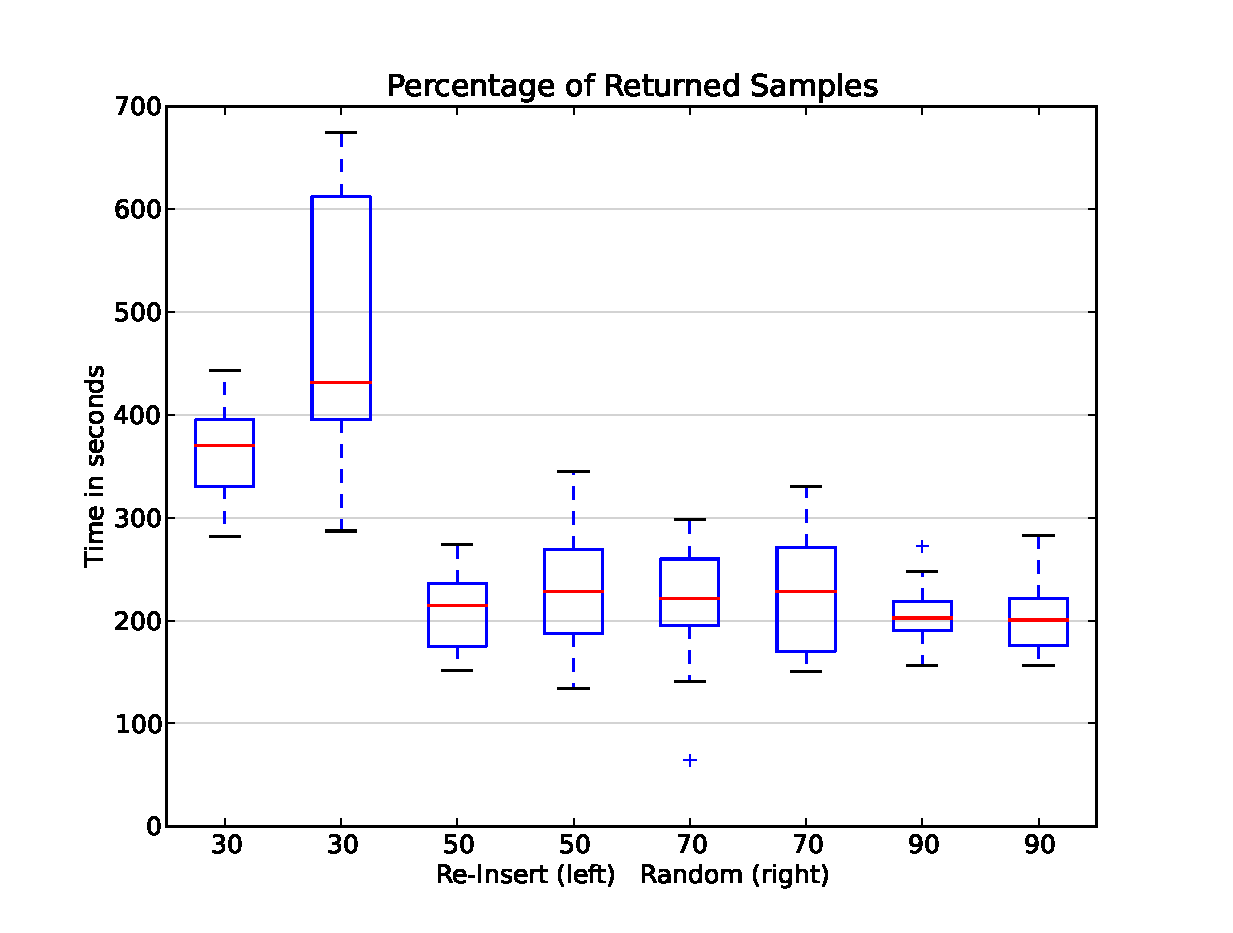
\includegraphics[width=5.5cm]{plot_time_CRS_w16.eps}
        \label{fig:plot_time_ri_w16}
    }
        \subfigure[]
    {
        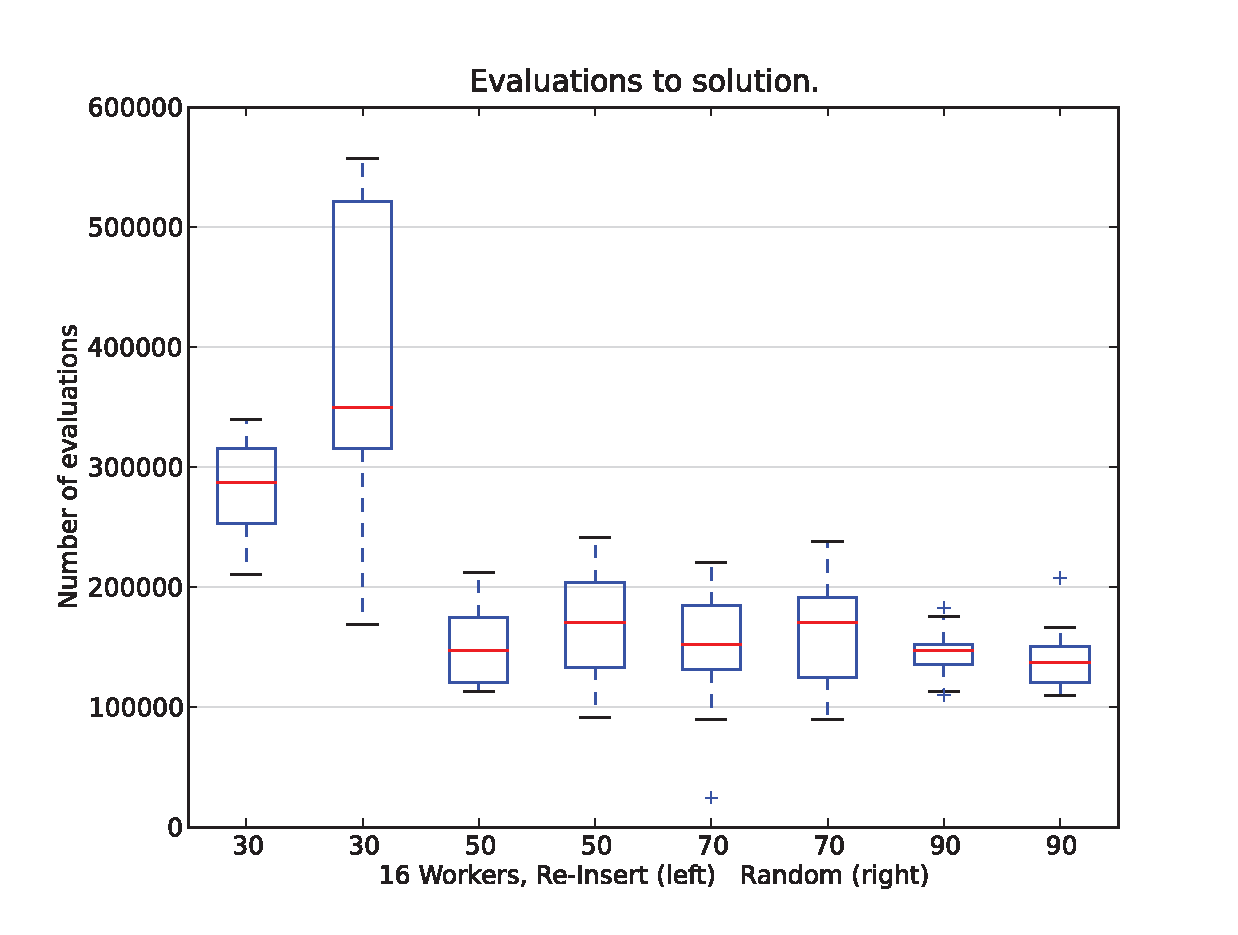
\includegraphics[width=5.5cm]{16_plot_evals.eps}
        \label{fig:plot_evals_w16}
    }
        \subfigure[]
    {
        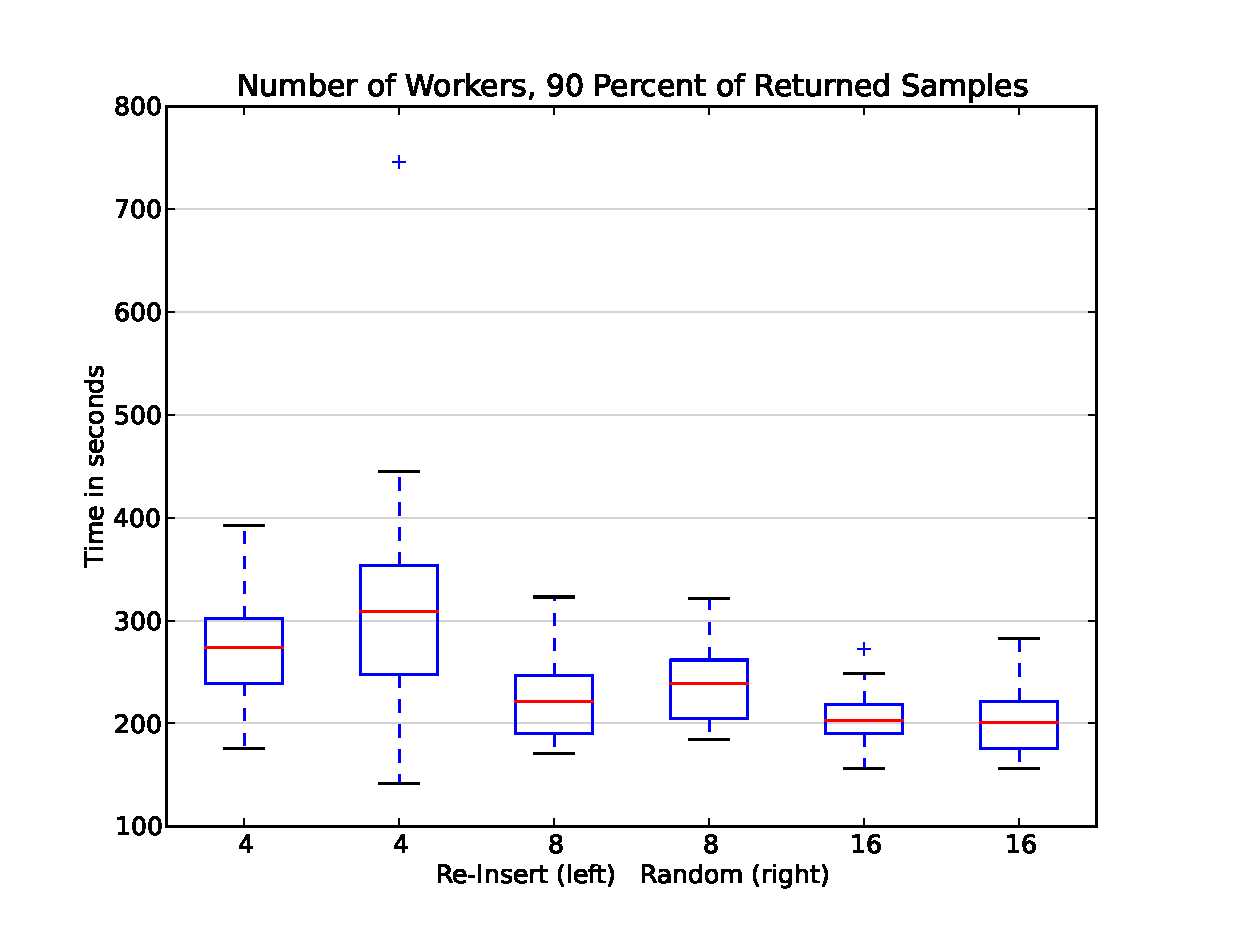
\includegraphics[width=5.5cm]{plot_percent_90.eps}
        \label{fig:plot_percent_90}
    }
        \subfigure[]
    {
        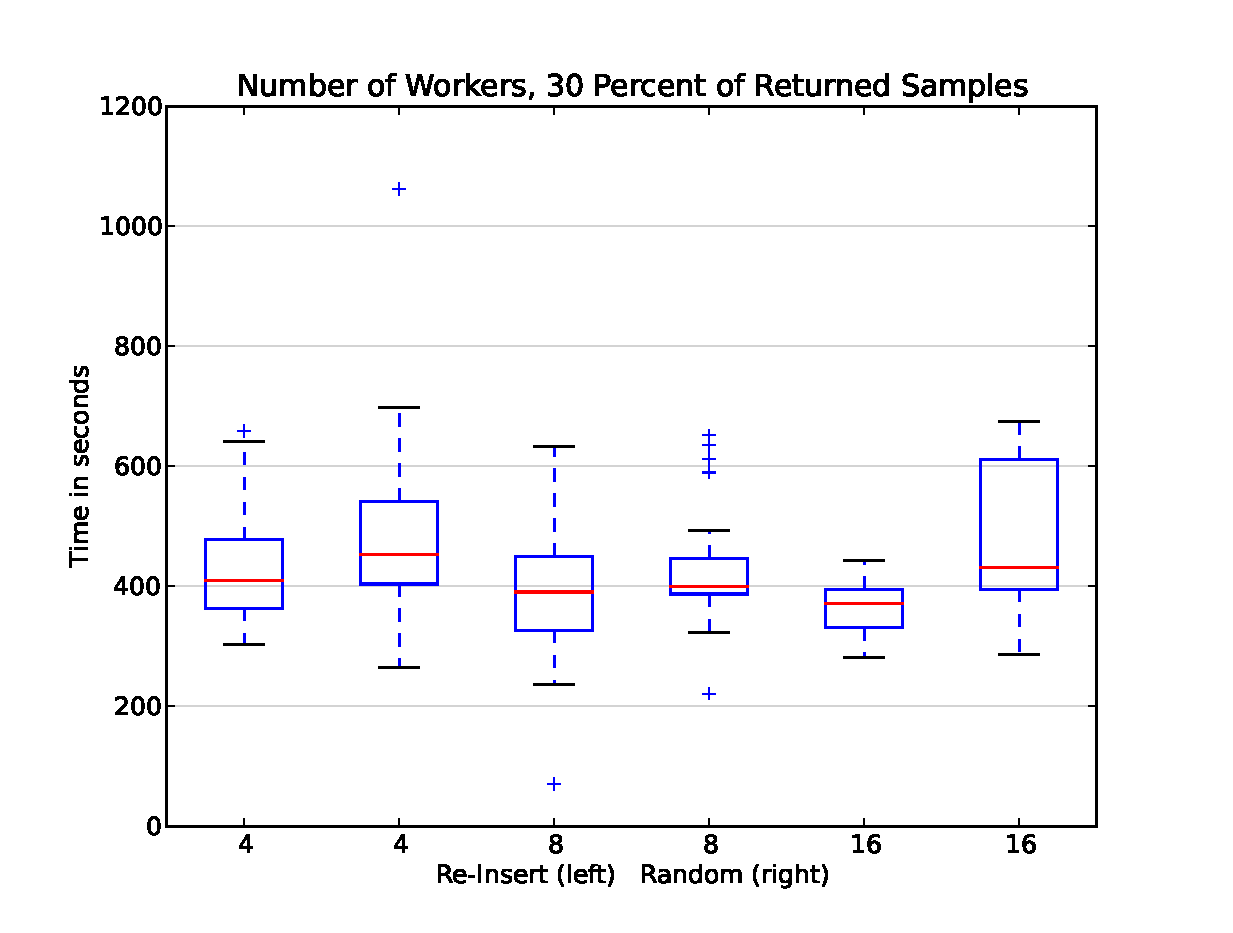
\includegraphics[width=5.5cm]{plot_percent_30.eps}
        \label{fig:plot_percent_30}
    }
        \subfigure[]
    {
        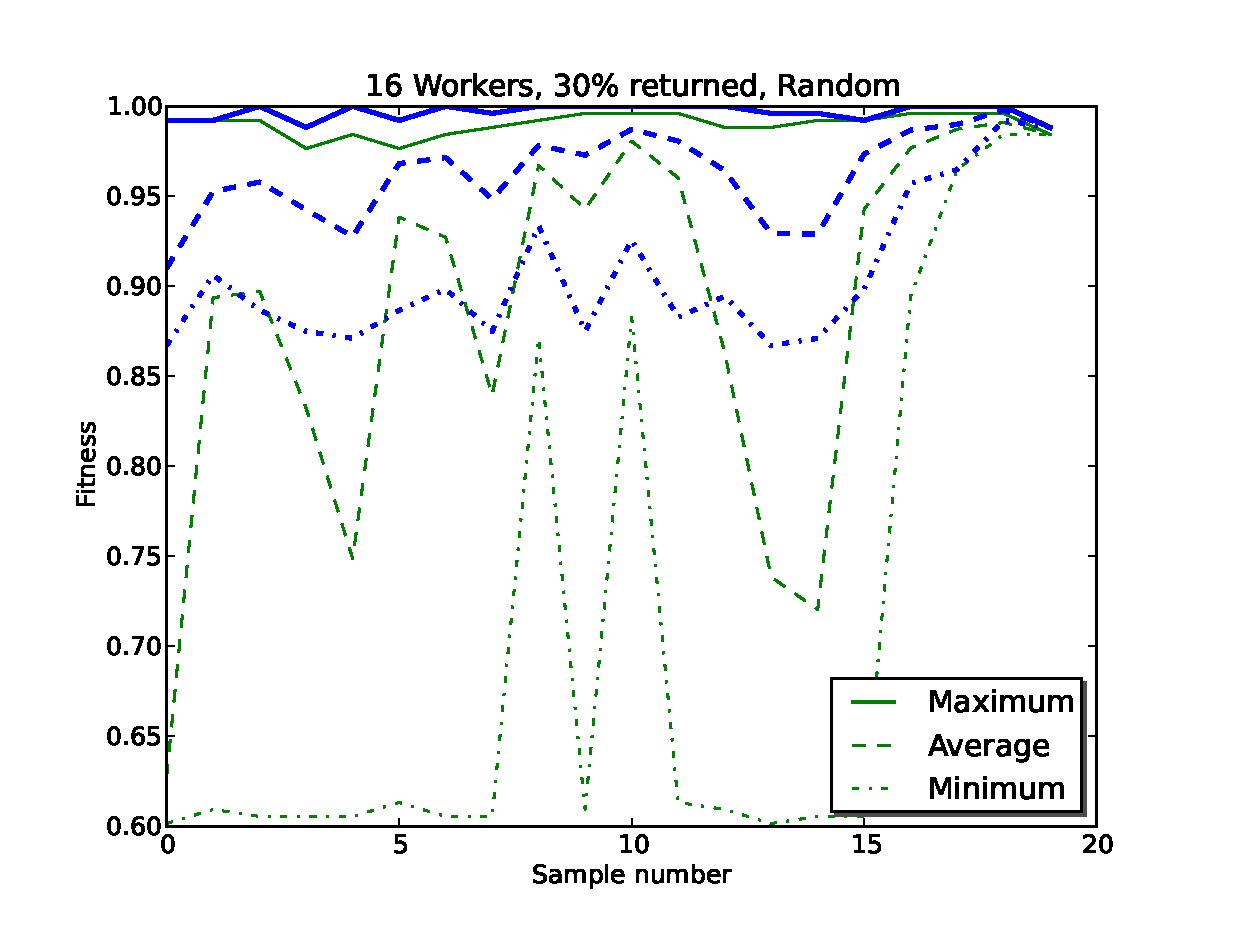
\includegraphics[width=5.5cm]{Fitness-w16-30-random.eps}
        \label{fig:Fitness-w16-30-random}
    }
        \subfigure[]
    {
        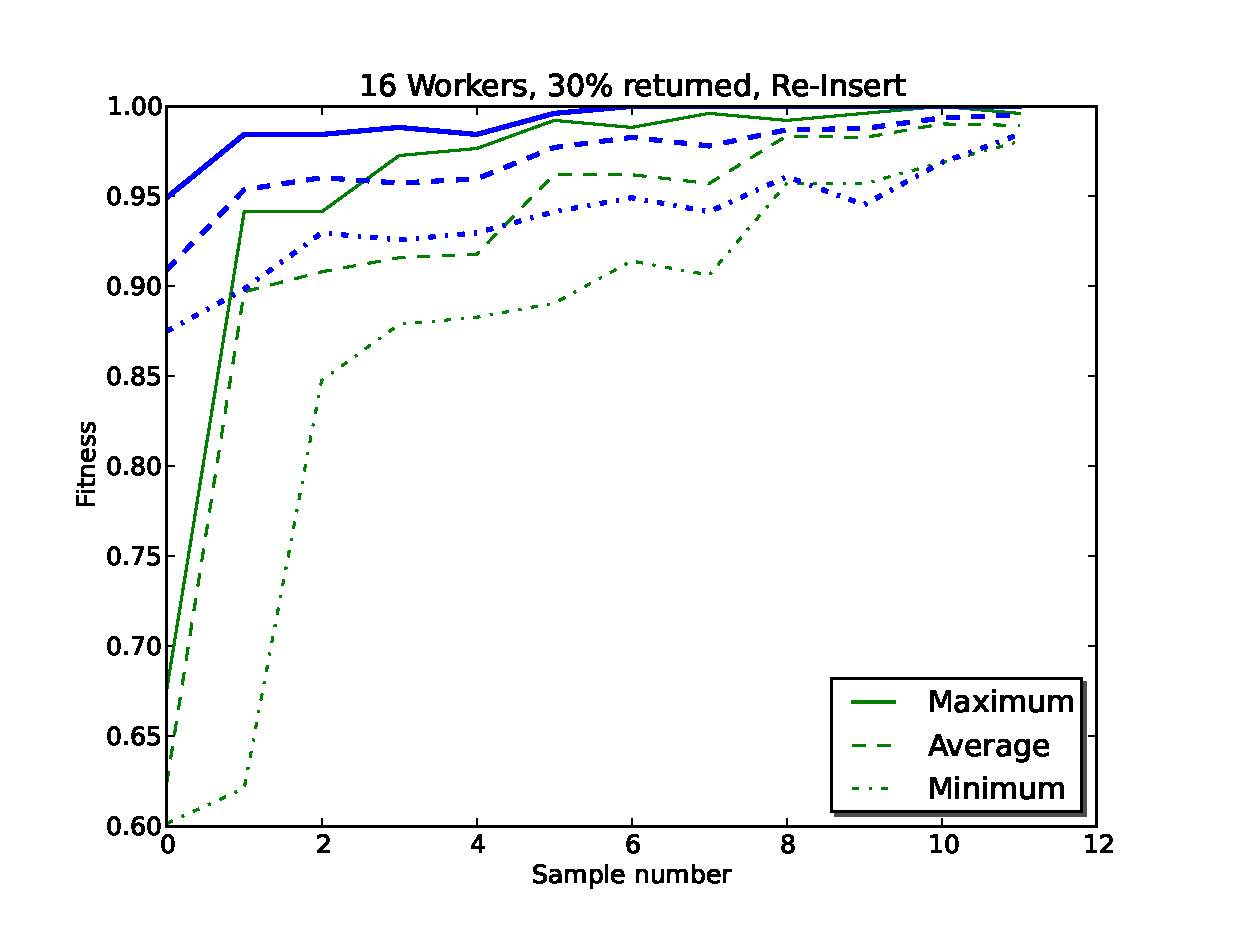
\includegraphics[width=5.5cm]{Fitness-w16-30-reinsert.eps}
        \label{fig:Fitness-w16-30-reinsert}
    }
    \caption{Unreliable workers: (a) Time to solution, 4 Workers; (b) Time to solution, 8 Worker;
    (c) Time to solution, 16 Workers; (d) Number of evaluations, 16 Workers; (e) Time to solution, 90\% returned samples;
    (f) Time to solution, 30\% returned samples; (g-h) Fitness by sample number, 30\% returned samples, 16 Workers,
    for each sample the average fitness was measured at the start (green) and at the end (blue) of the local evolution, with (g) random algorithm and
    (h) reinsertion algorithm.  }
    \label{fig:effort_unreliable}
\end{figure*}


This section evaluates the effect that the reinsertion algorithm has on the total
running time and number of evaluations of a GA, using the P-Peaks problem described above with the same parametrization.
In particular, two distinct approaches are evaluated: (a) reinserting previously taken individuals, at the cost of keeping copies of
samples; and (b) inserting randomly generated individuals, with has the added effect of increasing diversity within the population.

The algorithm stops when reaching the optimum value, or when all workers
pulled 100 samples. To simulate unreliable workers each worker was assigned a
return sample probability. In the experiments the lower probability was a 30\%
chance of an EvoWorker returning a sample or an EvoWorker failing 70\% of the
time; other return sample probabilities where 50\%, 70\% and 90\%. Experiments
where carried out for 4, 8 and 16 EvoWorkers.
Although supported by EvoSpace, time intervals were not chosen as triggers
to feed the population with new individuals, population size was used instead.
The population size is a better threshold as it is more critical
to a GA performance, for instance in experiments where the population remaining in the pool was near starvation, the time to completion increased.
For these experiments, the insertion of individuals was triggered when less than
128 individuals remain in the population; the number of individuals fed to the
population was 128, or 8 samples when the reinsertion algorithm was used.


Figure~\ref{fig:plot_time_ri_w4} shows the time required 
to solution when using four EvoWorkers. For a population of
512 individuals and a sample size of 16, there is no
difference in the time required to solution for 
percentages of 50\% and above. Both reinsertion algorithms
had comparable times. For 30 percent, both approaches 
had a slight increase in time. For 8 workers, shown in Figure~\ref{fig:plot_time_ri_w8},  there was a marginal
decrease in overall time; and results where similar to those found in the experiments with 4 workers.  
Figure~\ref{fig:plot_time_ri_w16} shows results for 16 workers,
when there was only a 30\% chance of returning a sample the rate of reinsertion was high, approximately once every 35 samples.
In this case, the insertion of random individuals resulted in a higher time to solution.
For these experiments when the rate of reinsertion is low, both alternatives
have similar results, but the reinsertion algorithm is better
for situations when starvation is common.
It appears that the insertion of random individuals is not detrimental when there
are other evolved individuals in the pool. But when the remaining
pool almost consists of random individuals, samples pulled by
EvoWorkers need to start the search from scratch. 
If a small number of samples are returned to the pool, the work needed to reach the
optimum is increased. Figure~\ref{fig:plot_evals_w16} also shows the number 
of evaluations needed to reach an optimum for 16 workers.
Figures~\ref{fig:plot_percent_90} and \ref{fig:plot_percent_30} show
the time required to solution for 30\% and 90\% of returned samples.
For 90\% both algorithms had similar speedups when the number of
workers is higher.
For 30\% there was practically no speedup at all. The reinsert algorithm,
although not significant, had a consistent decrease in time.         

Fitness with respect to time was measured as the average from each consecutive
sample pulled by each worker. For each sample the average fitness
was measured at the start and at the end of the local evolution.
Also the minimum and maximum fitness values at the start and finish was 
recorded.    
Figure~\ref{fig:Fitness-w16-30-random} shows the evolution of fitness
with the random insertion algorithm, where as expected initial fitness drops
at certain points, when random insertion occurs, while average final fitness 
is also compromised. Figure~\ref{fig:Fitness-w16-30-reinsert}
shows results for the reinsertion algorithm, with more
characteristic convergence curves without substantial fitness drops. 





\subsection{Parametrization}
In general, EAs are sometimes criticized by the large number of parameters they require,
that for real world problems need to be tuned empirically or require additional heuristic processes to be included into the search to
adjust the parameters automatically \cite{parameters,ss}.
In the case of a PEAs, this issue is magnified since the underlying system architecture adds several degrees of freedom to the search process,
with unknown interactions.
This problem is of particular importance in real-world scenarios, where there might be little prior insights regarding what could be the best
configuration for an EA tool, especially if the intent is to use it as a black-box optimizer;
a comprehensive survey on this topic is given in \cite{parameters}. 

A noteworthy contribution is made by Cant\'u Paz, who addresses the problem of deriving theoretical models of the effects
of parameters related to population size and migration in Island-Model EAs (IMEA) \cite{cantu}.
However, it does not cover the effects of all possible parameters, or the intricacies of a PEA algorithm.
Here, we would stress some important differences between PEAs and IMEAs.
First, an IMEA presents a fixed topological structure, with a predefined interaction protocol among each evolving population,
this leads to a coordinated, or even synchronized, interaction between the islands.
On the other hand, a PEA does not consider such a structure, the interactions between workers is much less structured or controlled.
Second, in an IMEA each island represents an individual evolutionary process, sharing some of the same dynamics as standard EAs.
In a PEA, however, only a single centralized population exists, samples of which are distributed across workers, but ultimately combined once again
in the centralized pool.
Therefore, some of the well-known insights derived from IMEA research (regarding, for example, migration policies) are not necessarily relevant in the PEA framework.

Therefore, the recent approach called Randomized Parameter Setting Strategy (RPSS) \cite{fuku1,fuku2} is tested with EvoSpace in this section.
The idea behind RPSS is that in a distributed EA, algorithm parametrization may be completely skipped to conduct a successful search.
The first works with RPSS focused on an IMEA model \cite{fuku1,fuku2}, that incorporates additional degrees of freedom that must be tuned before
performing a run.
Such a tuning task can become overwhelming, particularly if the number of islands is excessively large (hundreds).
Therefore, the proposal in \cite{fuku1} is to set the parameter values randomly, without a tuning or self-adaptive process whatsoever.
The RPSS approach sets the parameters of each deme randomly at the beginning of the run, a very simple and apparently naive approach.
Results suggest that when the number of distributed process is large enough, algorithm parameters can be set randomly and still achieve
good results.
Therefore the goal of this section is to evaluate RPSS on the EvoSpace PEA, which lacks the fixed population structure of an IMEA.

\begin{table}[!t]
\renewcommand{\arraystretch}{1.3}
\caption{GA and EvoWorker parameters for experiments.}
\label{tab:params}
\centering
\begin{tabular}{|l|c|}
\hline
\multicolumn{2}{|c|}{GA Parameters} \\
\hline
Tournament size & 4 \\
Crossover rate & 0.85  \\
Population Size & 512 \\
Mutation probability & 0.5 \\
Independent bit flip probability  & 0.02 \\
\hline
\multicolumn{2}{|c|}{EvoWorker Parameters} \\
\hline
Sample Size & 16 \\
Generations & 128 \\
\hline
\multicolumn{2}{|c|}{Other Parameters} \\
\hline
PiCloud Worker Type & Realtime \\
Number of Workers & 4,8,16 \\
Return Sample Probability & 30\%,50\%,90\% \\
Number of Executions & 30 \\

\hline

\end{tabular}
\end{table}

To gauge the effectiveness of RPSS on a PEA, it is compared with three different parametrization strategies, similar to what is done in \cite{fuku1,fuku2}.
All methods are compared based on average performance over a set of runs.
First, the simplest approach consists on setting all of the EvoWorker parameters homogeneously.
To do this, 200 random parametrizations are created, based on the ranges established in Table \ref{tab:params}.
The average performance of these runs characterizes the random-homogeneous parametrization, denoted Average-Homogeneous.
From these runs, the best configuration is chosen, the one that achieved the best results,
and then 20 independent runs are carried out on each problem, this method is called Best-Homogeneous.
However, here we use the Best-Homogeneous approach for direct comparison with \cite{fuku1,fuku2}.
Finally, the random-heterogeneous-parametrization is considered, where the parameters of each worker are set independently at random at
the beginning of each run; 20 independent runs are performed, the method is denoted as Average-Heterogeneous.
The algorithms are evaluated using the P-Peaks generator, as in previous sections.

Experiments are carried out using a different number of EvoWorkers $N$ on each problem.
The first group of runs are done with $N=16$ EvoWorkers, and the second with $N=120$.
Based on \cite{fuku1,fuku2}, it is assumed that with an increased number of workers the RPSS approach will achieve relatively better results, much closer to
the Best-Homogeneous configuration.
This is particularly important, since increasing the number of EvoWorkers greatly magnifies the dimensionality of the tuning problem.
while simplifying the tuning process
Results are summarized by tracking how the best solution found so far varies with respect to the total
number of samples taken from the EvoSpace pool of individuals.
These results are presented in Figure \ref{fig:PPeaks}, where the average performance for
each of the three methods evaluated here.

\begin{figure}[!ht]
    \centering
    	\subfigure[16 EvoWorkers]
    {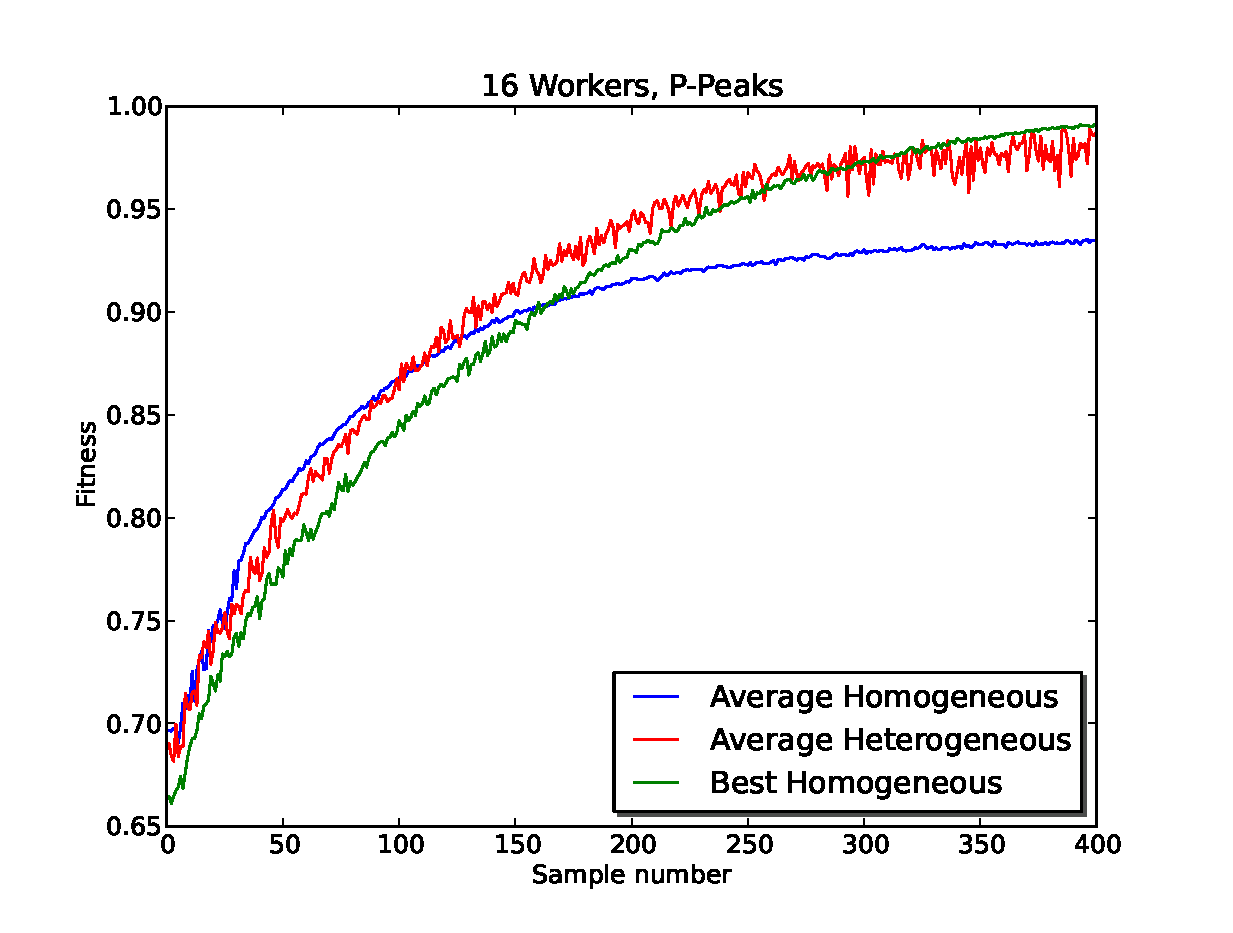
\includegraphics[width=6cm]{PPeaks-w16.eps}}
        \subfigure[120 EvoWorkers]
    {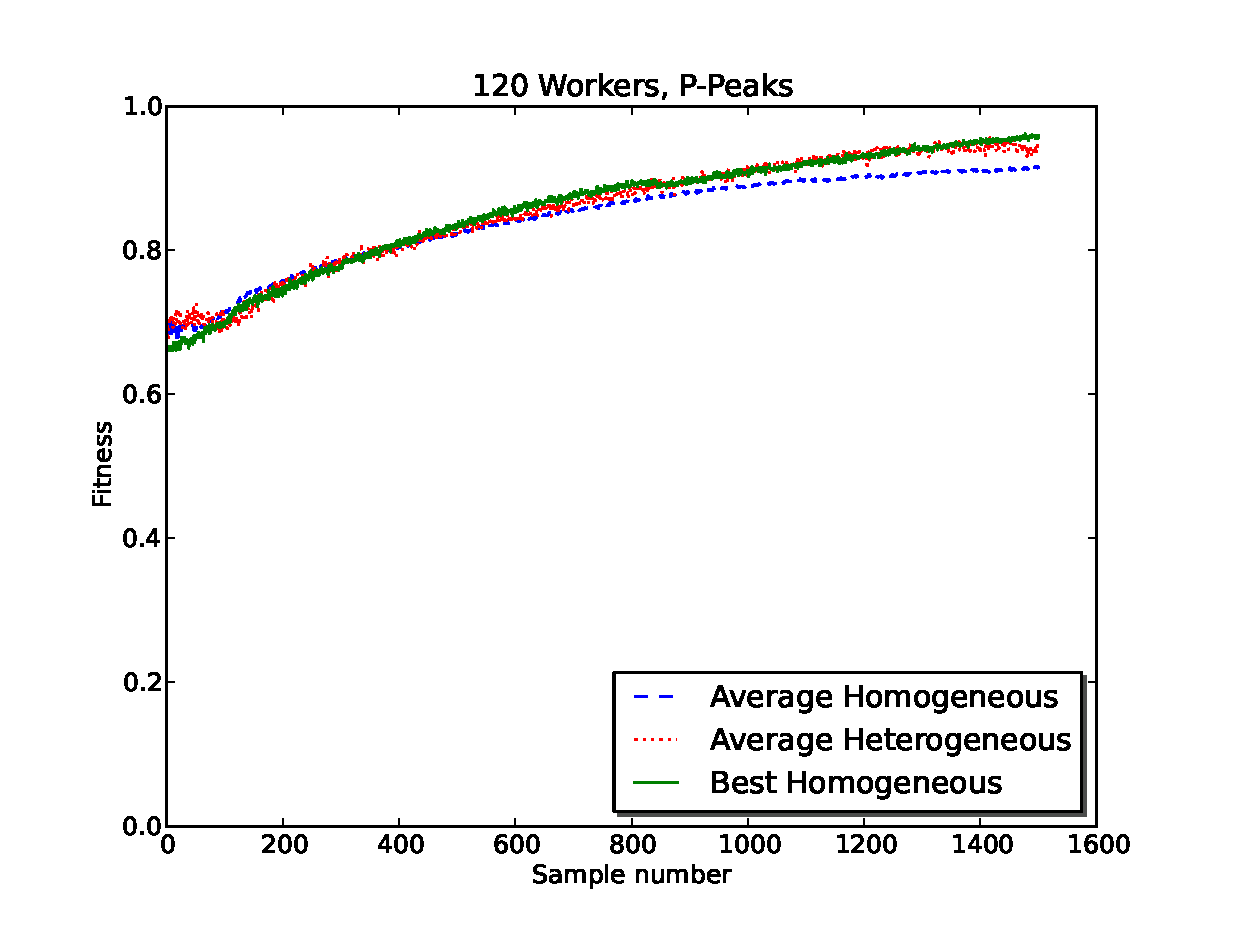
\includegraphics[width=6cm]{PPeaks-w120.eps}}
    \caption{Convergence plots for the P-Peaks with 16 (a) and 120 (b) EvoWorkers .}
    \label{fig:PPeaks}
\end{figure}



First, for the P-Peaks problem with 16 EvoWorkers.
In this case, we can see a clear trend, the random Heterogeneous configuration is very similar with the best homogeneous configuration,
depicted in Figure \ref{fig:PPeaks}(a).
This is a promising initial observation, since the heterogeneous configuration did not require any parameter tuning, while the best homogeneous configuration
is chosen from a set of 200 runs.
Moreover, we see that using an homogeneous configuration with random values achieves noticeably inferior performance.
When the number of EvoWorkers is increased, shown in Figure \ref{fig:PPeaks}(b), a similar trend appears,
however the differences among the algorithms is reduced.
Nevertheless, it is obvious that using a random heterogeneous parametrization can be used as an off-the shelf approach for EvoSpace parametrization.



\subsection{Discussion}


\section{Concluding Remarks}
\label{sec:conclusions}




%\begin{acknowledgements}
%If you'd like to thank anyone, place your comments here
%and remove the percent signs.
%\end{acknowledgements}

% BibTeX users please use one of
%\bibliographystyle{spbasic}      % basic style, author-year citations
%\bibliographystyle{spphys} 



\bibliographystyle{spmpsci}      % mathematics and physical sciences
%\bibliographystyle{spphys}       % APS-like style for physics

\bibliography{biblio}   % name your BibTeX data base
\end{document}
% end of file template.tex

